\documentclass{sigchi}

% Use this section to set the ACM copyright statement (e.g. for
% preprints).  Consult the conference website for the camera-ready
% copyright statement.

% Copyright
\CopyrightYear{2016}
%\setcopyright{acmcopyright}
\setcopyright{acmlicensed}
%\setcopyright{rightsretained}
%\setcopyright{usgov}
%\setcopyright{usgovmixed}
%\setcopyright{cagov}
%\setcopyright{cagovmixed}
% DOI
\doi{http://dx.doi.org/10.475/123_4}
% ISBN
\isbn{123-4567-24-567/08/06}
%Conference
\conferenceinfo{CHI'16,}{May 07--12, 2016, San Jose, CA, USA}
%Price
\acmPrice{\$15.00}

% Use this command to override the default ACM copyright statement
% (e.g. for preprints).  Consult the conference website for the
% camera-ready copyright statement.

%% HOW TO OVERRIDE THE DEFAULT COPYRIGHT STRIP --
%% Please note you need to make sure the copy for your specific
%% license is used here!
% \toappear{
% Permission to make digital or hard copies of all or part of this work
% for personal or classroom use is granted without fee provided that
% copies are not made or distributed for profit or commercial advantage
% and that copies bear this notice and the full citation on the first
% page. Copyrights for components of this work owned by others than ACM
% must be honored. Abstracting with credit is permitted. To copy
% otherwise, or republish, to post on servers or to redistribute to
% lists, requires prior specific permission and/or a fee. Request
% permissions from \href{mailto:Permissions@acm.org}{Permissions@acm.org}. \\
% \emph{CHI '16},  May 07--12, 2016, San Jose, CA, USA \\
% ACM xxx-x-xxxx-xxxx-x/xx/xx\ldots \$15.00 \\
% DOI: \url{http://dx.doi.org/xx.xxxx/xxxxxxx.xxxxxxx}
% }

% Arabic page numbers for submission.  Remove this line to eliminate
% page numbers for the camera ready copy
% \pagenumbering{arabic}

% Load basic packages
\usepackage{balance}       % to better equalize the last page
\usepackage{graphics}      % for EPS, load graphicx instead 
\usepackage[T1]{fontenc}   % for umlauts and other diaeresis
\usepackage{txfonts}
\usepackage{mathptmx}
\usepackage[pdflang={en-US},pdftex]{hyperref}
\usepackage{color}
\usepackage{booktabs}
\usepackage{textcomp}

% Some optional stuff you might like/need.
\usepackage{microtype}        % Improved Tracking and Kerning
% \usepackage[all]{hypcap}    % Fixes bug in hyperref caption linking
\usepackage{ccicons}          % Cite your images correctly!
% \usepackage[utf8]{inputenc} % for a UTF8 editor only

% If you want to use todo notes, marginpars etc. during creation of
% your draft document, you have to enable the "chi_draft" option for
% the document class. To do this, change the very first line to:
% "\documentclass[chi_draft]{sigchi}". You can then place todo notes
% by using the "\todo{...}"  command. Make sure to disable the draft
% option again before submitting your final document.
\usepackage{todonotes}


% Custom Stuff
\graphicspath{{figures/}{pictures/}{images/}{./}}
\newcommand{\figref}[1]{\hyperref[#1]{Figure~\ref*{#1}}}
\usepackage{xspace}
\newcommand{\ie}{{i.e.}\xspace}
\newcommand{\eg}{{e.g.,}\xspace}
\newcommand{\cf}{{c.f.}\xspace}
\newcommand{\ea}{{et~al.}\xspace}
\newcommand{\aka}{{a.k.a.}\xspace}
\newcommand{\etc}{{etc.}\xspace}
\hyphenation{LayerCake}

\usepackage{subcaption}
\usepackage{amsmath}
\usepackage{hyperref}


% Paper metadata (use plain text, for PDF inclusion and later
% re-using, if desired).  Use \emtpyauthor when submitting for review
% so you remain anonymous.
\def\plaintitle{Value-Suppressing Uncertainty Palettes}
\def\plainauthor{Anonymous}
\def\emptyauthor{}
\def\plainkeywords{Uncertainty Visualization; Color Perception; Thematic Maps; Semiotics.}
\def\plaingeneralterms{Uncertainty Visualization, Color Perception}

% llt: Define a global style for URLs, rather that the default one
\makeatletter
\def\url@leostyle{%
  \@ifundefined{selectfont}{
    \def\UrlFont{\sf}
  }{
    \def\UrlFont{\small\bf\ttfamily}
  }}
\makeatother
\urlstyle{leo}

% To make various LaTeX processors do the right thing with page size.
\def\pprw{8.5in}
\def\pprh{11in}
\special{papersize=\pprw,\pprh}
\setlength{\paperwidth}{\pprw}
\setlength{\paperheight}{\pprh}
\setlength{\pdfpagewidth}{\pprw}
\setlength{\pdfpageheight}{\pprh}

% Make sure hyperref comes last of your loaded packages, to give it a
% fighting chance of not being over-written, since its job is to
% redefine many LaTeX commands.
\definecolor{linkColor}{RGB}{6,125,233}
\hypersetup{%
  pdftitle={\plaintitle},
% Use \plainauthor for final version.
%  pdfauthor={\plainauthor},
  pdfauthor={\emptyauthor},
  pdfkeywords={\plainkeywords},
  pdfdisplaydoctitle=true, % For Accessibility
  bookmarksnumbered,
  pdfstartview={FitH},
  colorlinks,
  citecolor=black,
  filecolor=black,
  linkcolor=black,
  urlcolor=linkColor,
  breaklinks=true,
  hypertexnames=false
}

% create a shortcut to typeset table headings
% \newcommand\tabhead[1]{\small\textbf{#1}}

% End of preamble. Here it comes the document.
\begin{document}

\title{\plaintitle}

%Figure list:
% Vsum vs. traditional 2D heatmap vs. juxtaposed maps
% Chart of color bins w/r/t CIELAB threshold, with iconic maps at intervals
% Process figure
% Real examples with different color maps




\newcommand{\teaserFig}{
  \teaser{
		\centering
		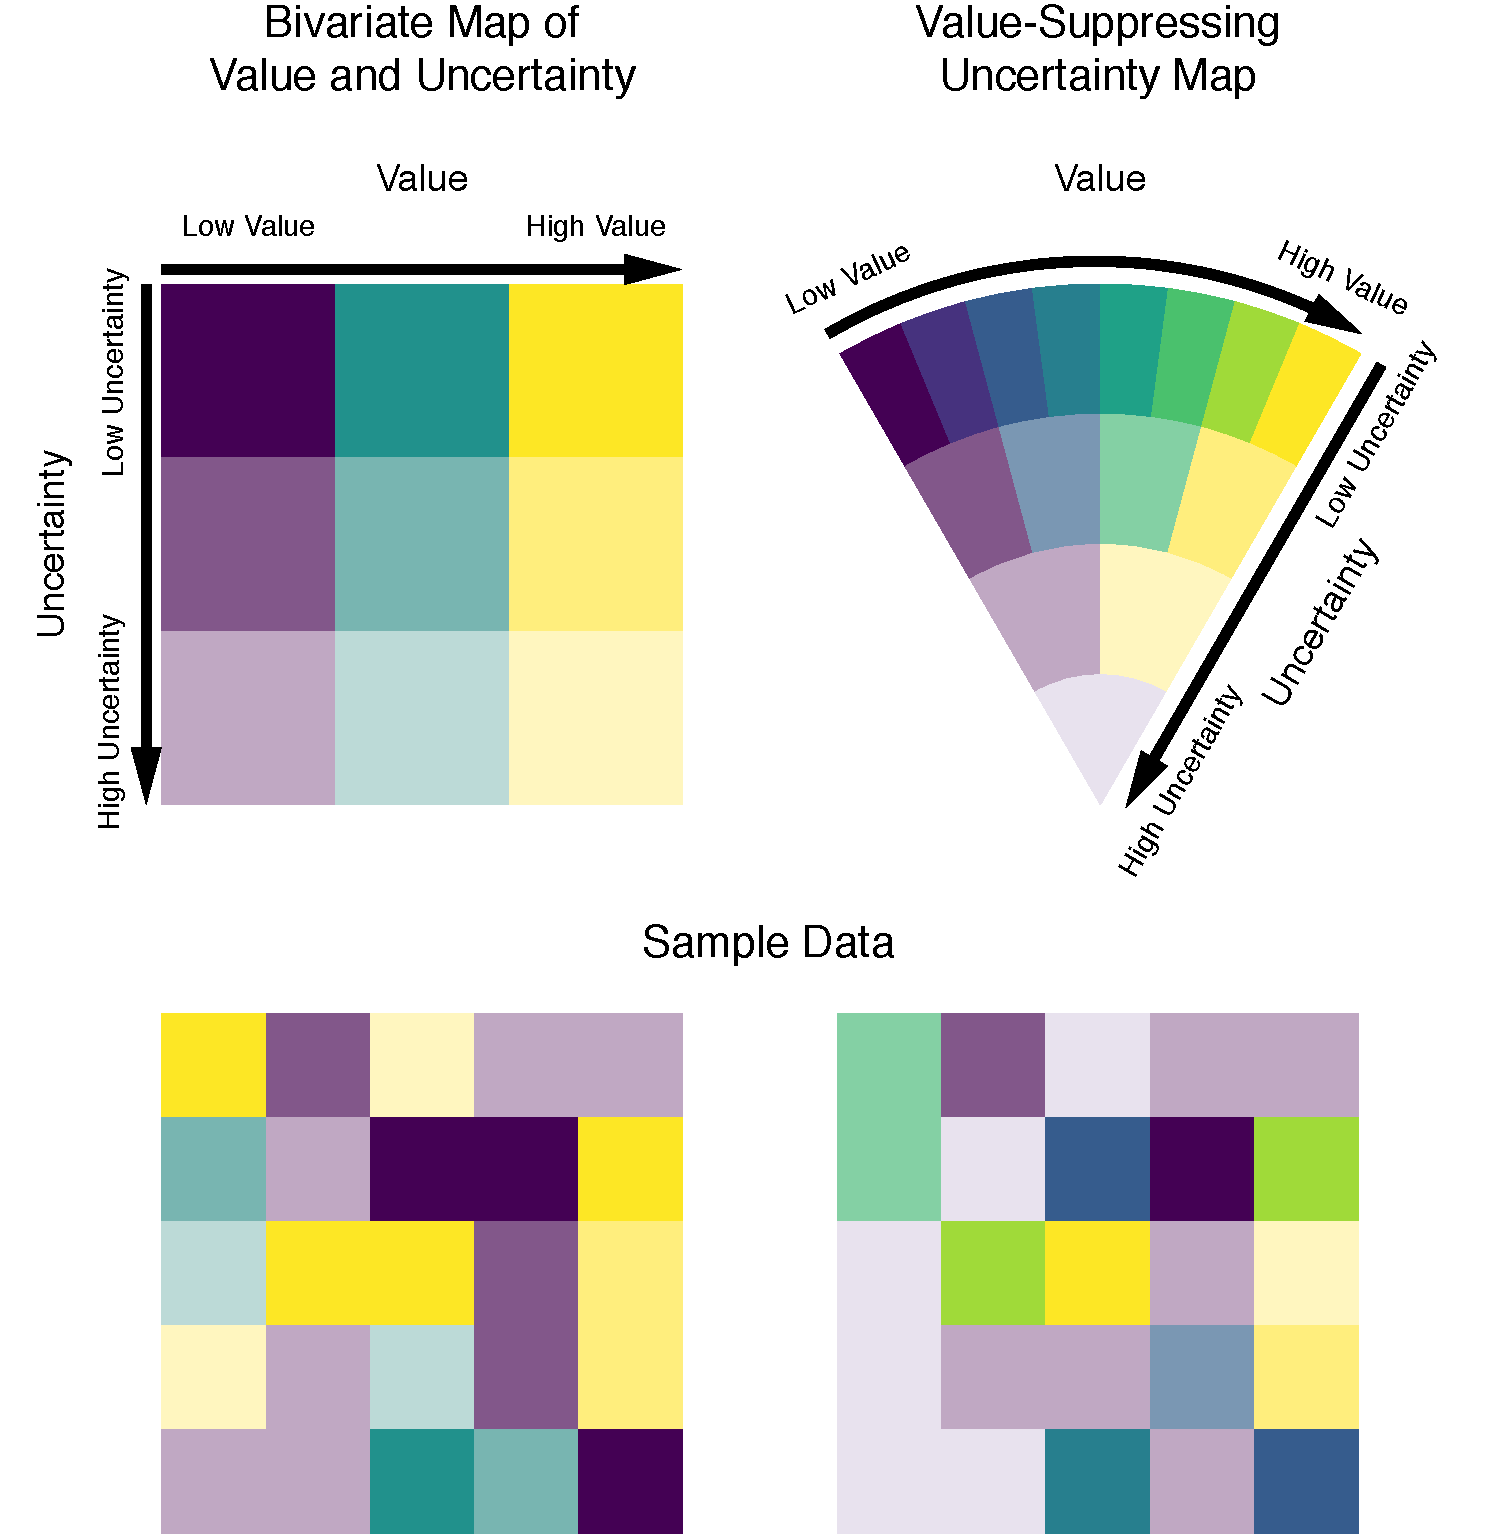
\includegraphics[width=0.9\textwidth]{example.pdf}
		\caption{Lookit! Lookit!}
		\label{fig:teaser}
	}
}

\newcommand{\exampleFig}{
\begin{figure}[t]
	\centering
	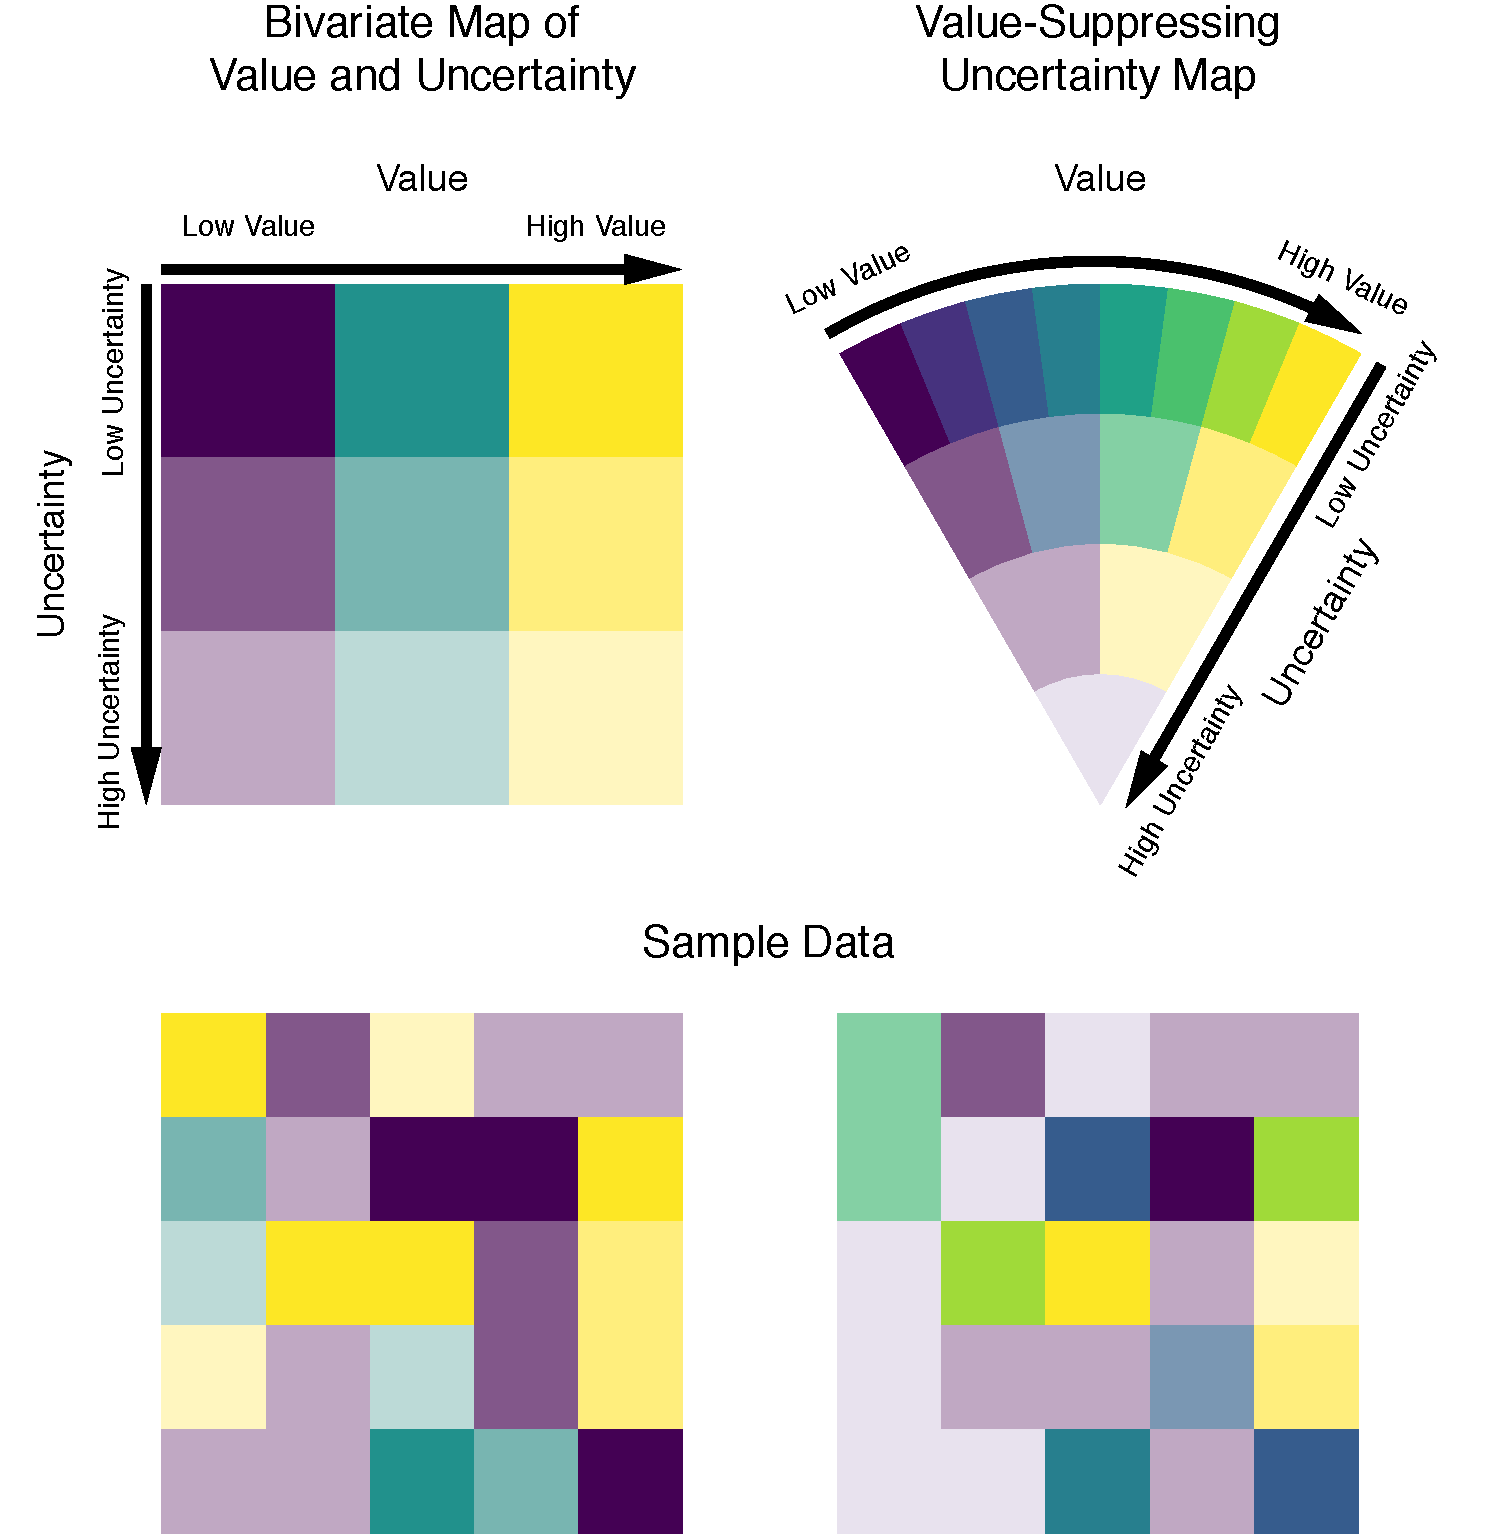
\includegraphics[width=0.9\columnwidth]{example.pdf}
	\caption{A standard bivariate map (left) and a VSUM (right), used to encode an identical 5x5 grid of random data. Both use the same visual channels to encode value (position along the Viridis~\cite{viridis} color map) and uncertainty (lightness and saturation), and have an equal standard of perceptual discriminability (at least 18 units of distance in CIELAB color space between colors). However, highly uncertain values result in colors that are very close together in the bivariate case, meaning the full bivariate map is only 9 bins under these constraints\,---\,a 4x4 map would result in colors that are perceptually too close together. By contrast, the VSUM intentionally reduces bins when uncertainty is high, eventually aliasing all highly uncertain values to the same color. This decision affords more distinct colors in other regions of the map, and so an increase in overall bins to 15. The resulting map suppresses the value of highly uncertain data, but increases the discriminability of data with low uncertainty.}
	\label{fig:example}
\end{figure}
}

\newcommand{\sizeFig}{
	\begin{figure}
		\centering
		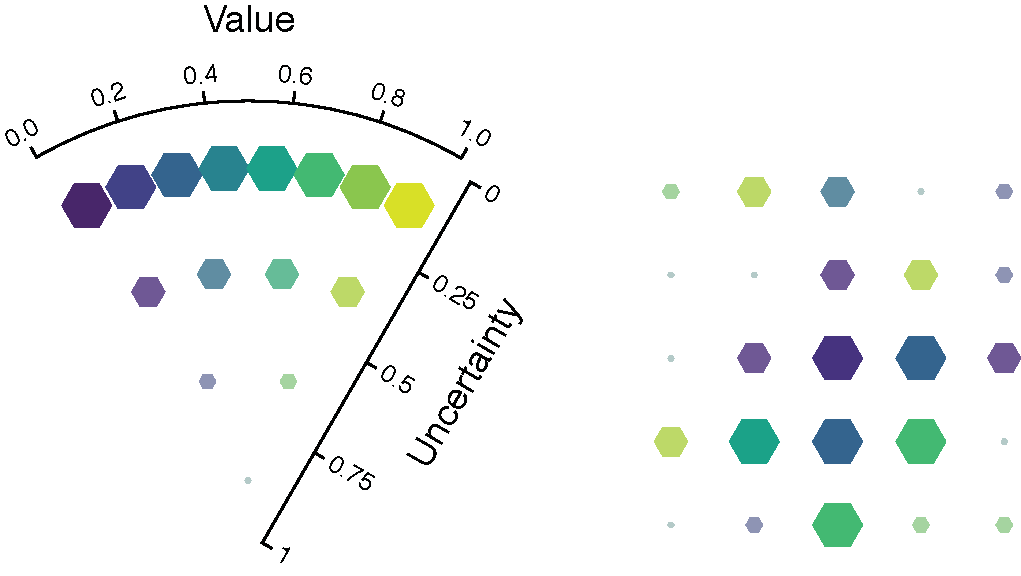
\includegraphics[width=0.9\columnwidth]{size.pdf}
		\caption{A VSUM where value is mapped to color, and uncertainty is mapped to glyph area. As glyphs become smaller, it becomes more difficult to distinguish their colors~\protect\cite{stone2014engineering}. VSUMs, by reducing the number of color categories as uncertainty increases, account for this ambiguity. On the right, the VSUM has been used to encode a 5x5 grid of random data.}
		\label{fig:size}
	\end{figure}
}

\newcommand{\conditionFig}{
	\begin{figure*}[t]
		\centering
		\begin{subfigure}{0.3\textwidth}
			\centering
			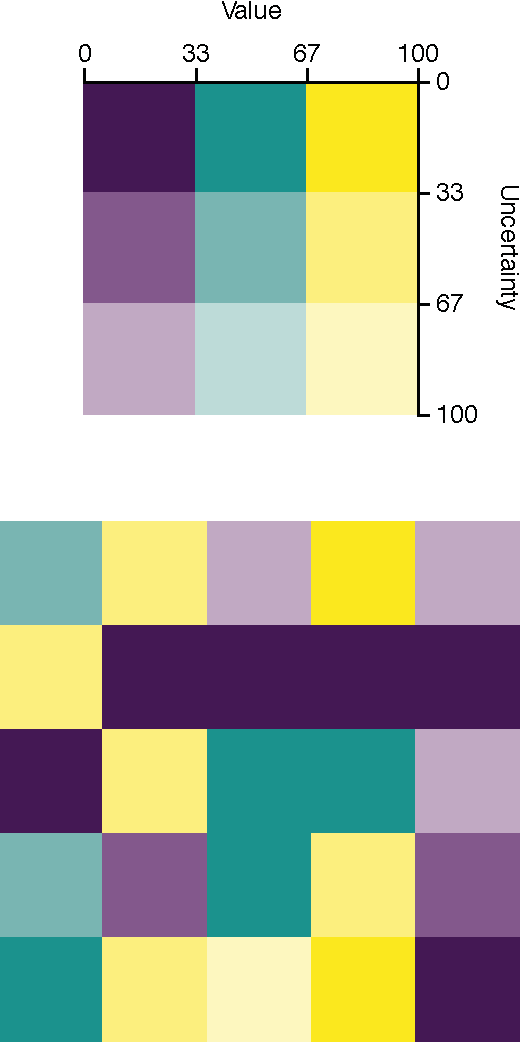
\includegraphics[width=.45\textwidth]{conditions1.pdf}
			\caption{Traditional Bivariate Map}
		\end{subfigure}
		~
		\begin{subfigure}{0.3\textwidth}
			\centering
			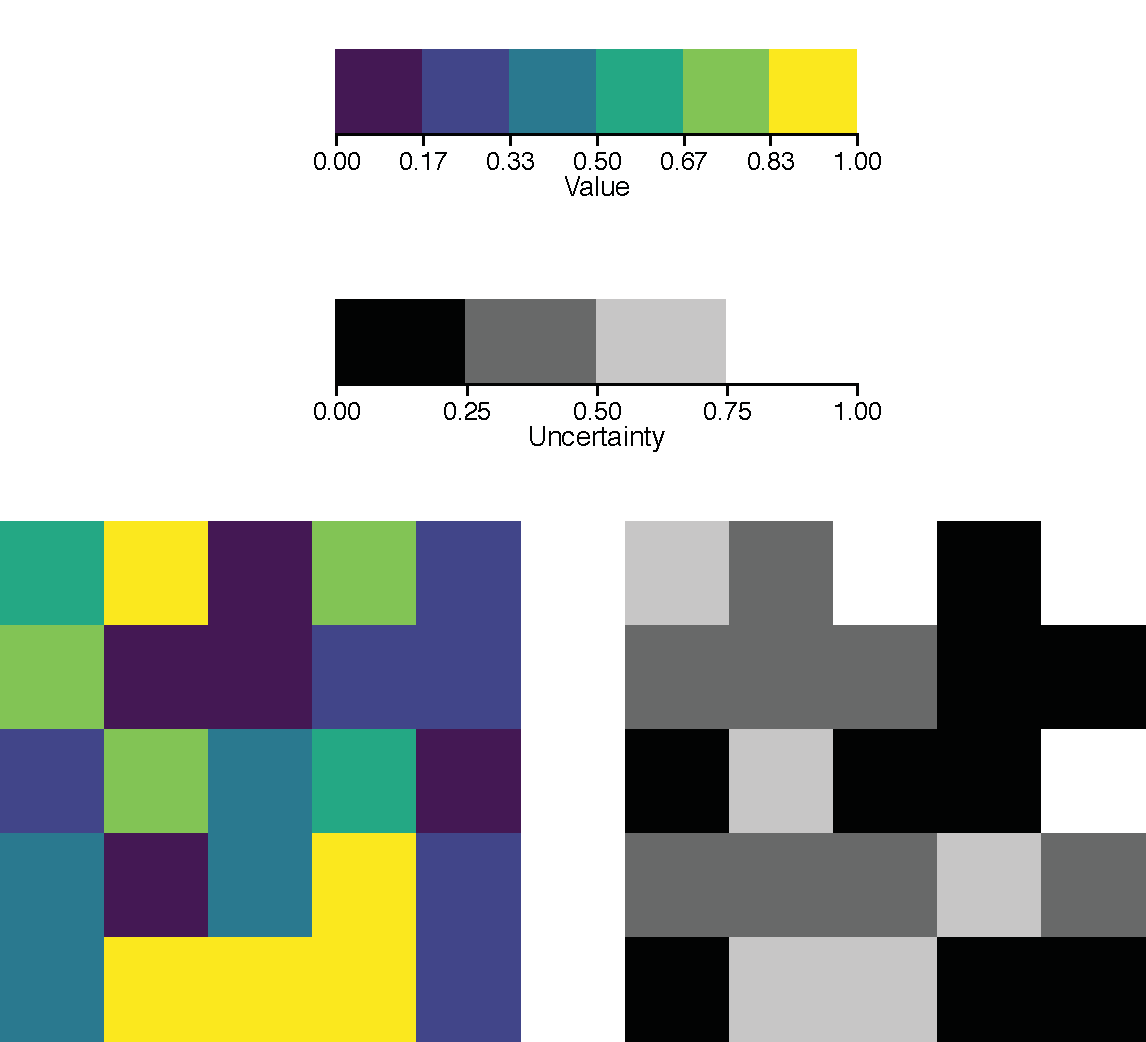
\includegraphics[width=\textwidth]{conditions2.pdf}
			\caption{Juxtaposed Univariate Maps}
		\end{subfigure}
		~
		\begin{subfigure}{0.3\textwidth}
			\centering
			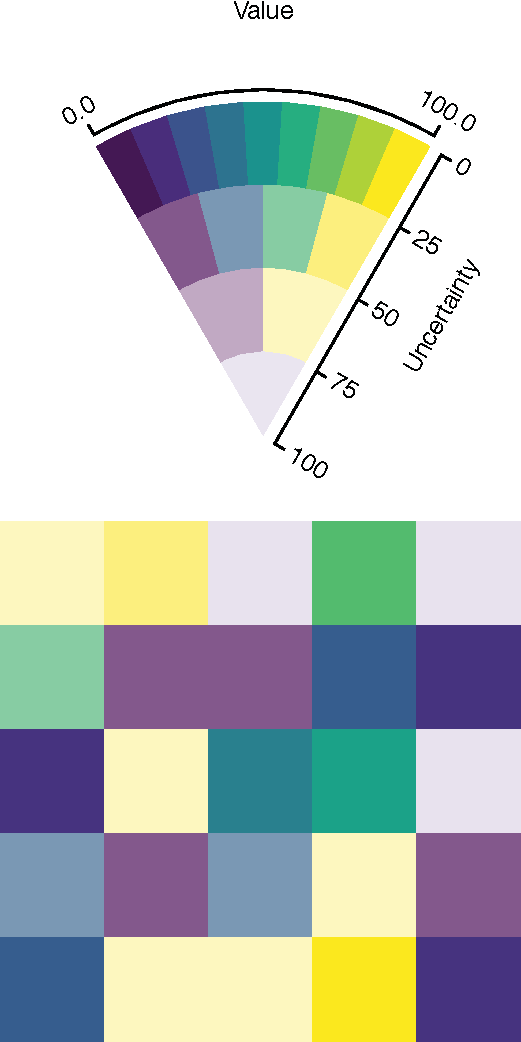
\includegraphics[width=0.45\textwidth]{conditions3.pdf}
			\caption{Value-Suppressing Uncertainty Map}
		\end{subfigure}
		\caption{The three graph types in our evaluation. Bivariate color ramps ensure that there are orthogonal mappings for each combination of value and uncertainty, but, since color channels are not separable, can afford only a few discrete colors before color categories become unacceptably close, perceptually. Juxtaposed maps, by keeping these channels separate, afford a larger range of colors, but require a visual search task to recover both value and uncertainty in a region. VSUMs have many of the advantages of bivariate maps, but assign more color categories to certain data, at the expense of ambiguity when uncertainty is high.}
		\label{fig:conditions}
	\end{figure*}
}

\newcommand{\taskTwoFig}{
	\begin{figure*}
		\centering
		\begin{subfigure}{0.45\textwidth}
			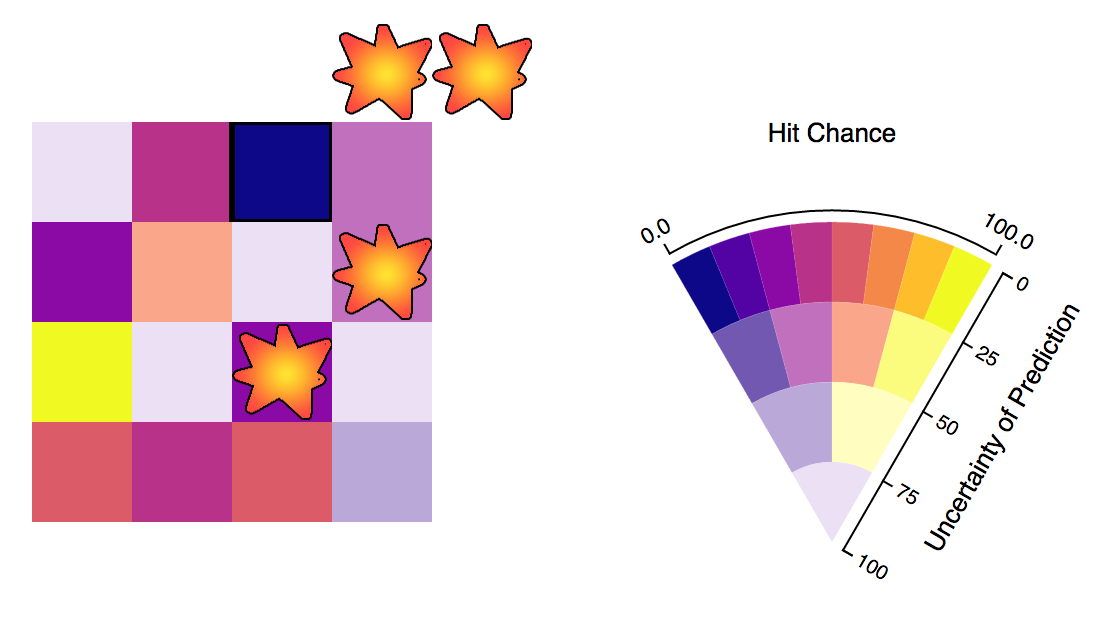
\includegraphics[width=\textwidth]{attack.png}
			\caption{Attacking}
			\label{fig:taskTwoAttack}
		\end{subfigure}
		~
		\begin{subfigure}{0.45\textwidth}
			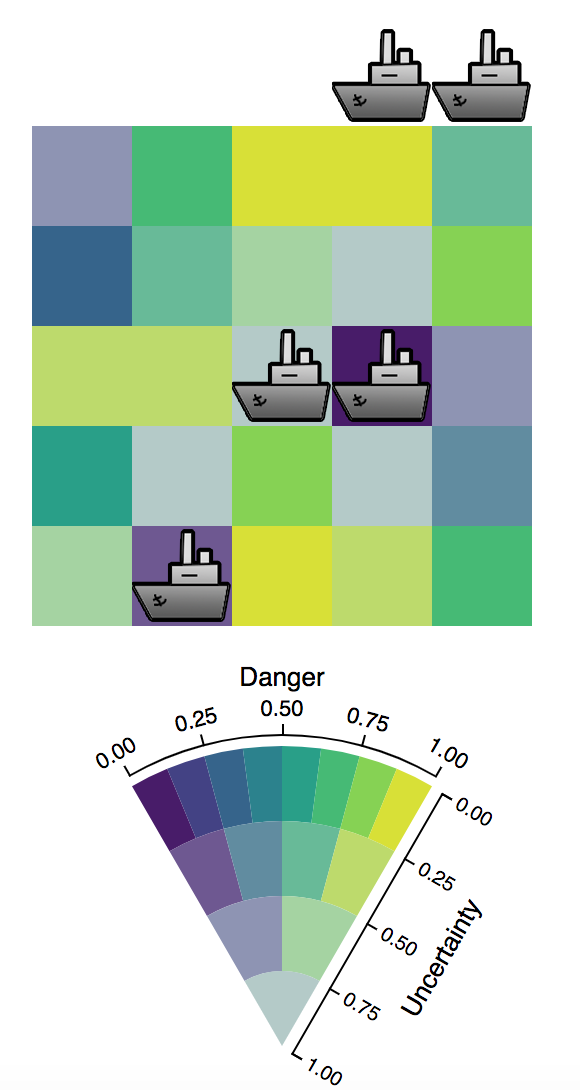
\includegraphics[width=\textwidth]{defend.png}
			\caption{Defending}
			\label{fig:taskTwoDefend}
		\end{subfigure}
		\caption{The two framings of the Prediction task. In the ``attack'' framing, the participant is given a map of predictions of the location of enemy ships, along with the uncertainty in those predictions. The participant should place their missile strikes on locations with a high probability of containing a ship, and with high certainty in this probability. The ``defend'' framing is the opposite task: the participant has a list of likely missile locations, and ought to place their ships on locations with low probability of attack, and high certainty in this probability.}
		\label{fig:taskTwoConditions}
	\end{figure*}
}

\newcommand{\performanceFig}{
	\begin{figure}[t]
		\centering
		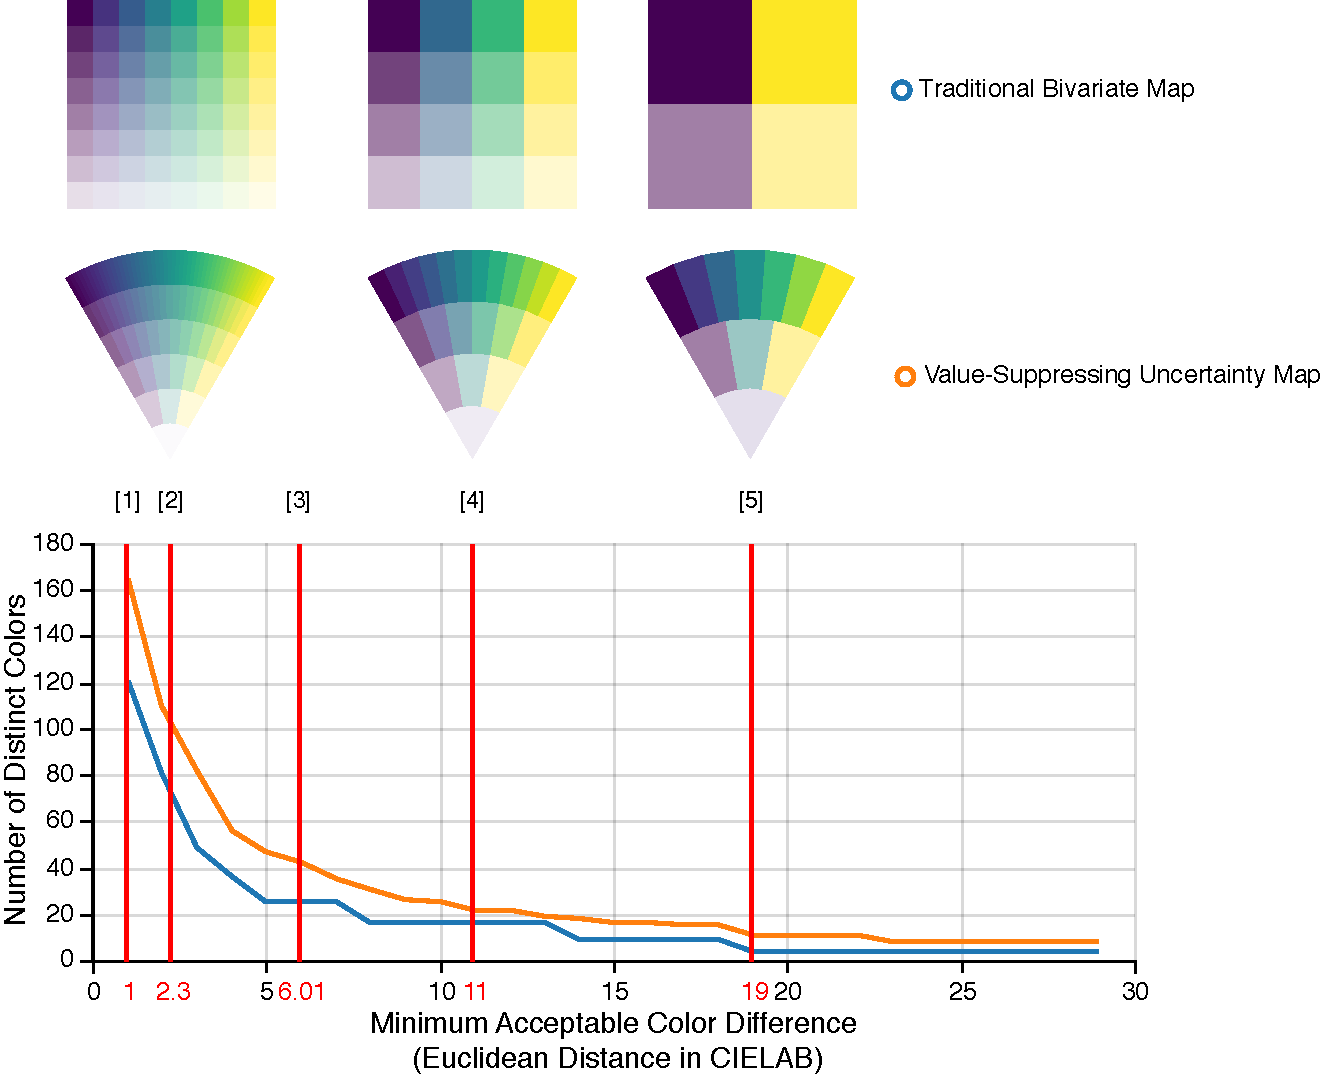
\includegraphics[width=0.9\columnwidth]{performance.pdf}
		\caption{
			The number of discrete color categories in traditional bivariate color maps versus VSUMs, assuming value is encoded by the Viridis color map~\protect\cite{viridis}, and uncertainty is encoded by saturation/value (whiter values are more uncertain). Since these whiter uncertain colors are closer together in CIELAB space, and VSUMs intentionally require fewer color bins in those regions, VSUMs always have more color categories than the corresponding 2D bivariate map. The red lines denote:
		  \textbf{1)} Theoretical 50\% JND from CIELAB specification.
			\textbf{2)} 50\% JND from controlled lab study of Mahy et al.~\protect\cite{mahy1994evaluation}.
			\textbf{3)} 50\% JND from Szafir et al.\protect\cite{szafir2014adapting}.
			\textbf{4)} 50\% JND for small visual targets from Stone et al.~\protect\cite{stone2014engineering}.
			\textbf{5)} The threshold resulting in the simplest possible (2x2) bivariate map.
	    }
		\label{fig:performance}
	\end{figure}
}

\newcommand{\flowFig}{
	\begin{figure}[t]
		\centering
		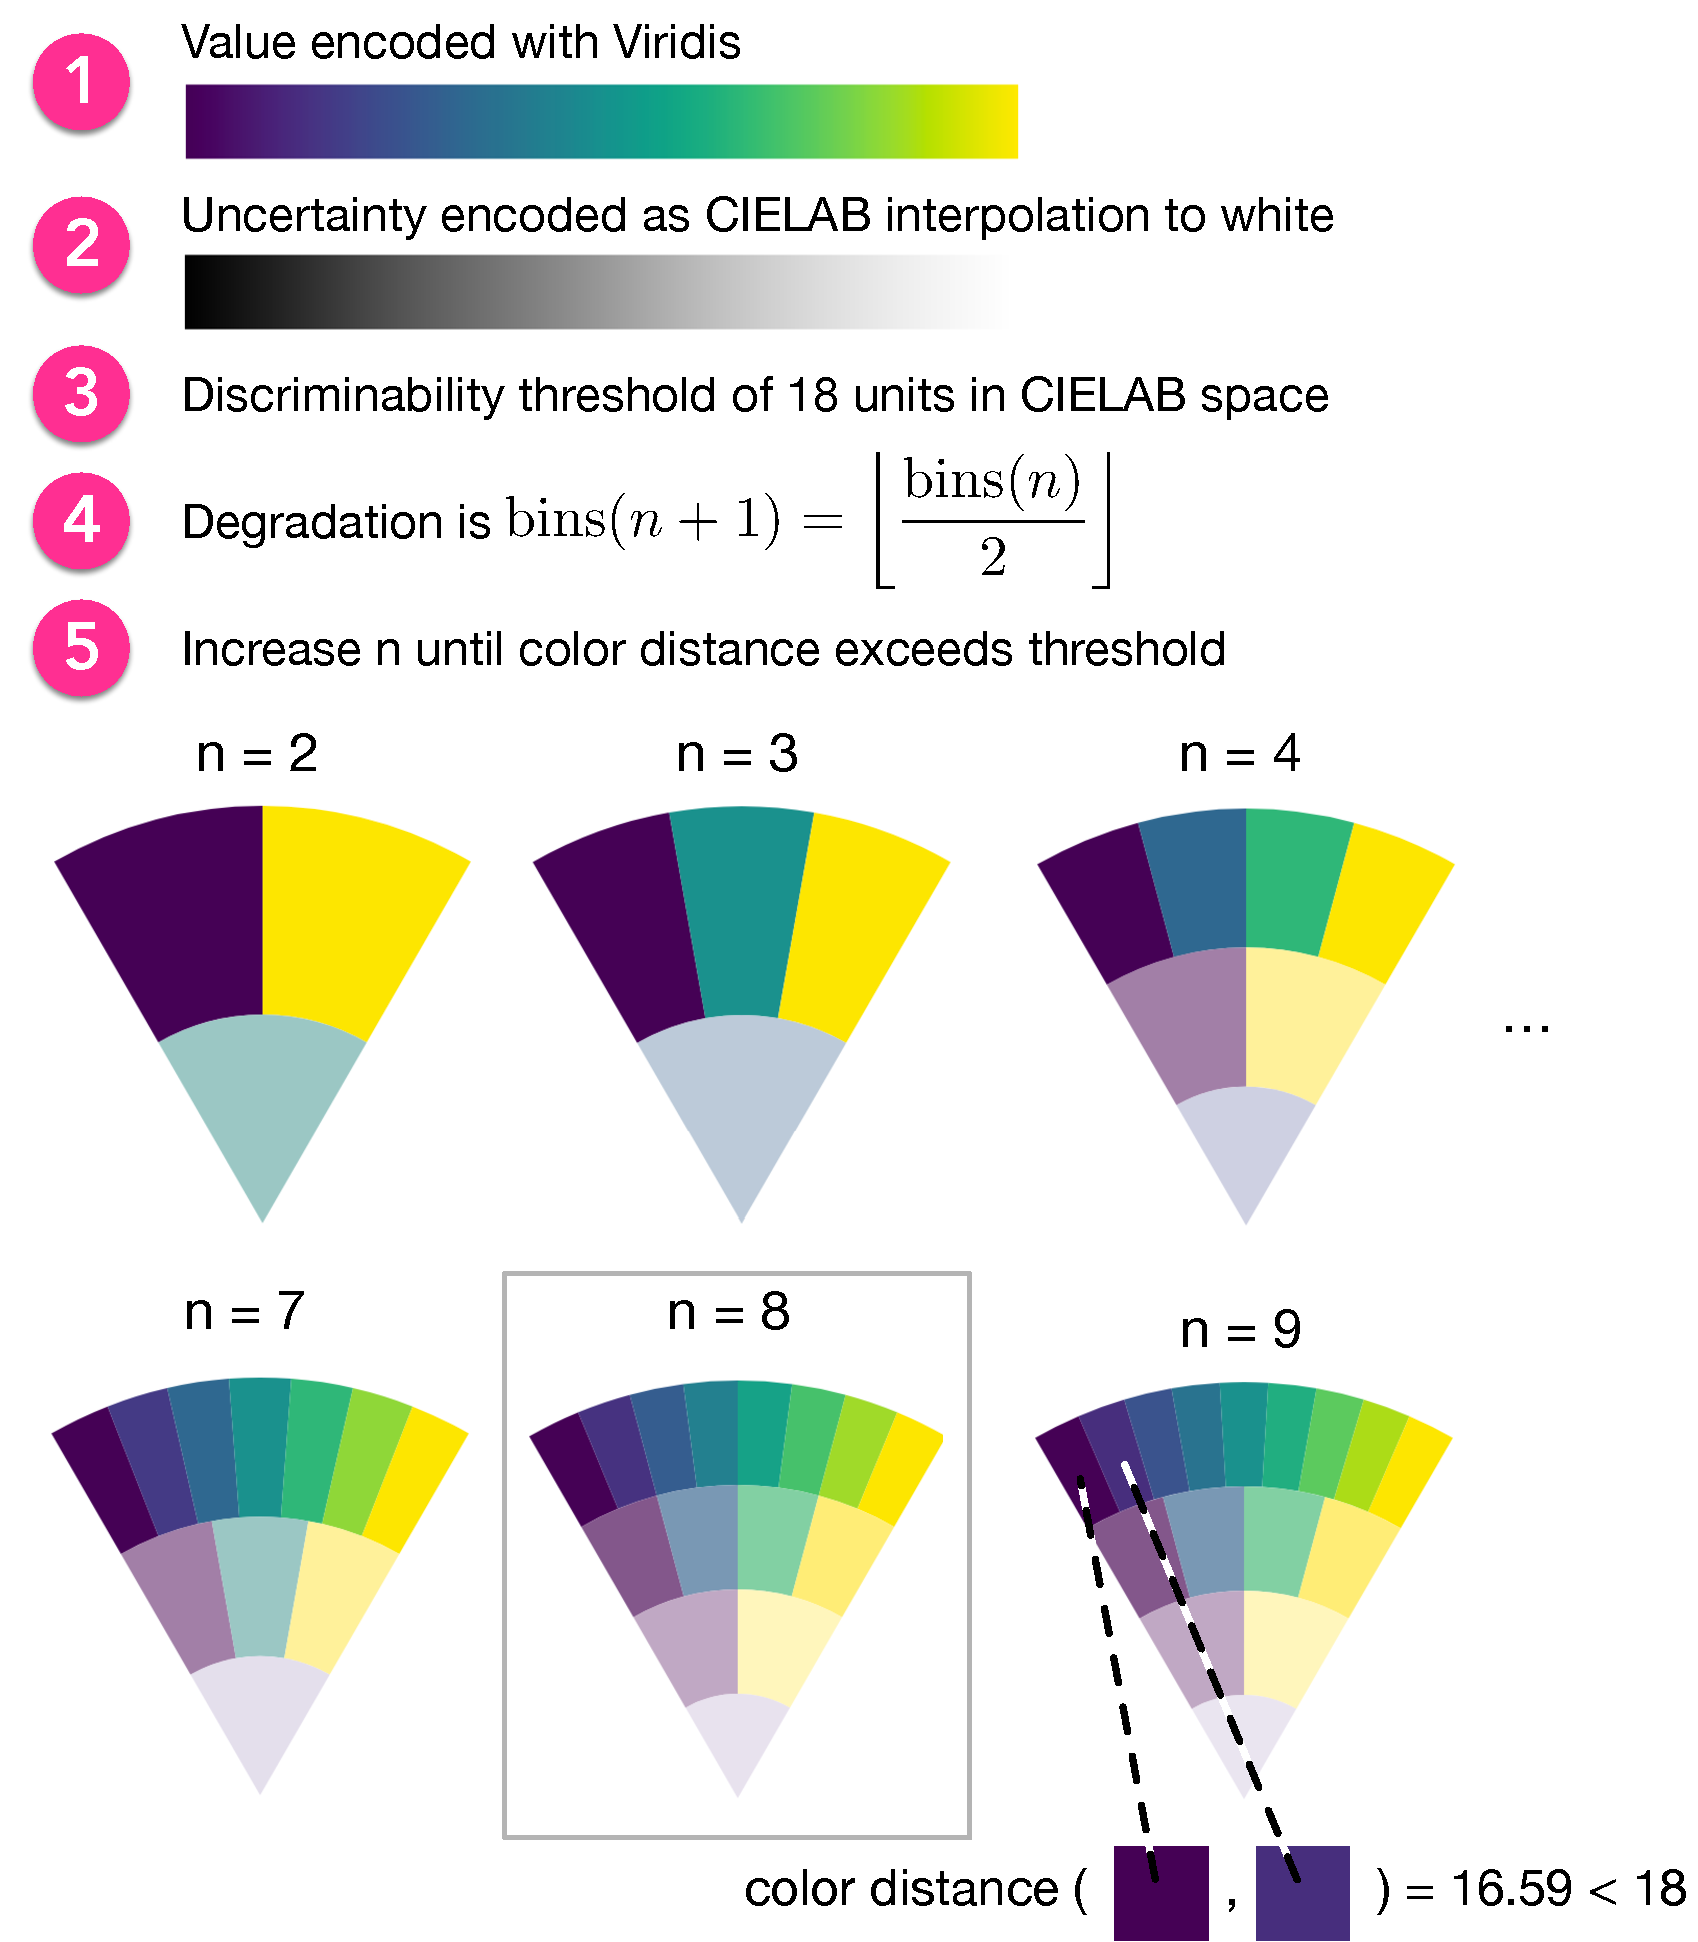
\includegraphics[width=0.95\columnwidth]{flow.pdf}
		\caption{The process for creating a VSUM. VSUMs guarantee that no two marks in the resulting bivariate mapping are perceptually closer than some pre-specified threshold. This guarantee removes some of the issues of non-separability and ambiguity that are otherwise a concern when designing bivariate maps. \\
		In this example two colors from the map for $n=9$ are too close in CIELAB space. Thus, we create a VSUM with $n=8$ color bins at the lowest level of uncertainty.}
		\label{fig:flow}
	\end{figure}
}

\newcommand{\airlineFig}{
\begin{figure}[t]
	\centering
	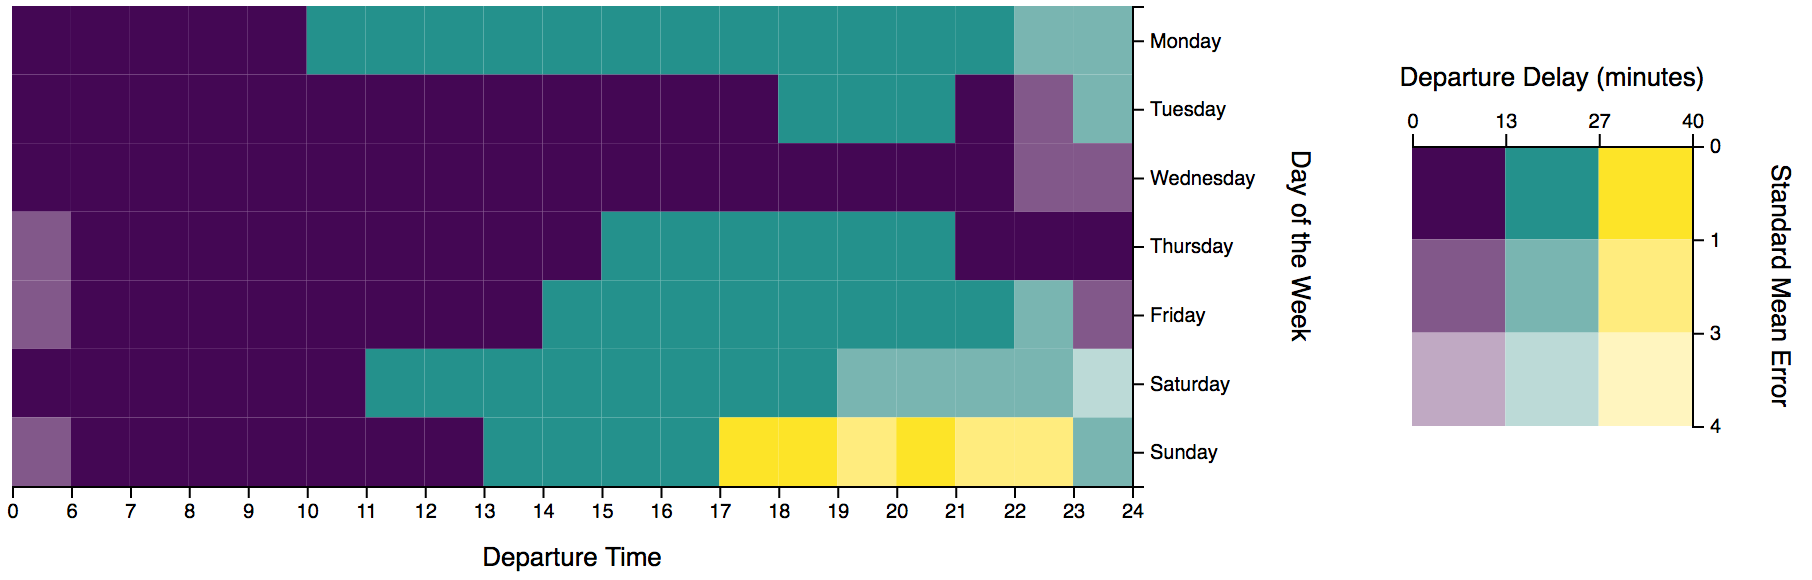
\includegraphics[width=\columnwidth]{airline-2d.png}
	\vspace{-15px}
	\caption{Average departure delay for different times of the day and days of the week visualized with a 2D uncertainty map. Horizontal position is the hour of scheduled departure, and vertical position is the day of the week.}
	\label{fig:airline2d}

	\vspace{10px}

	\centering
	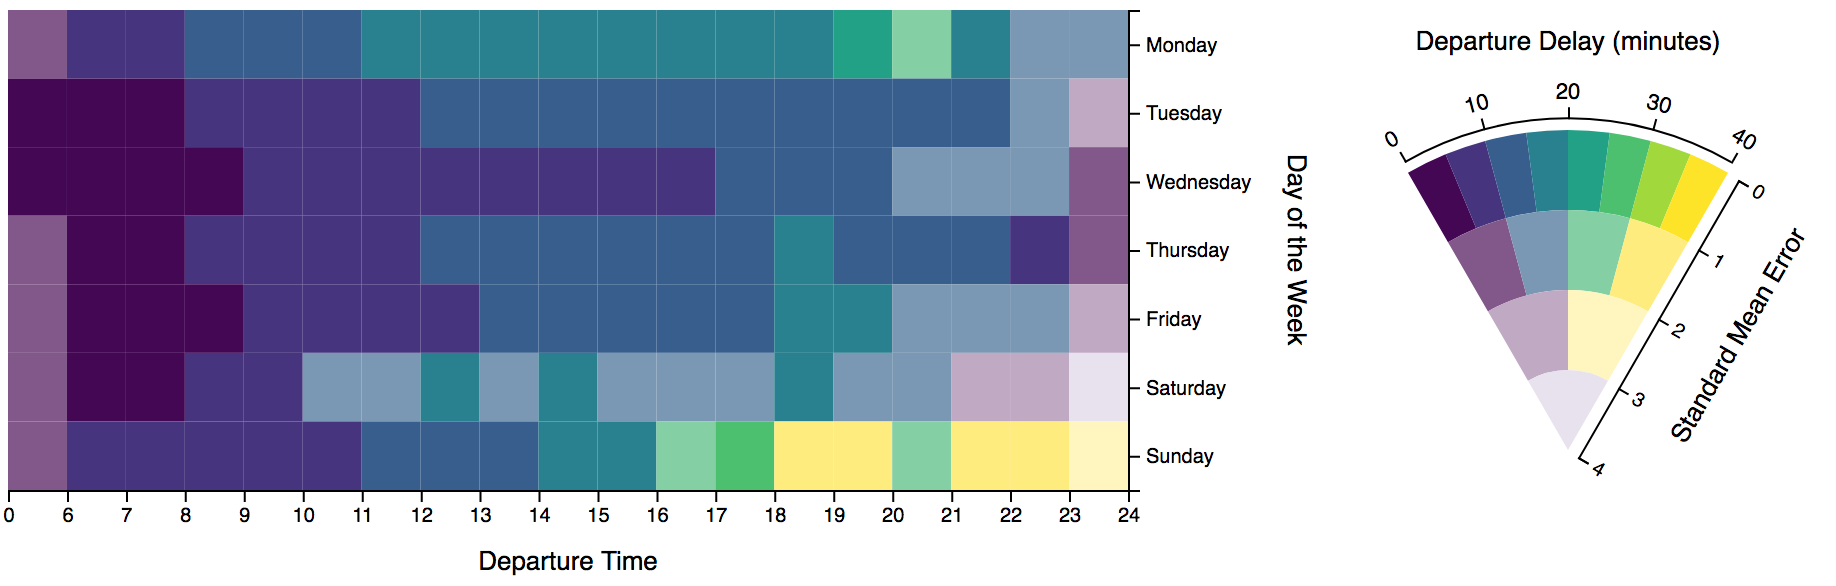
\includegraphics[width=\columnwidth]{airline-vsum.png}
	\vspace{-15px}
	\caption{Flight delay data encoded with a VSUM.}
	\label{fig:airlineVsum}
\end{figure}
}

\newcommand{\viralFig}{
\begin{figure}[t]
	\centering
	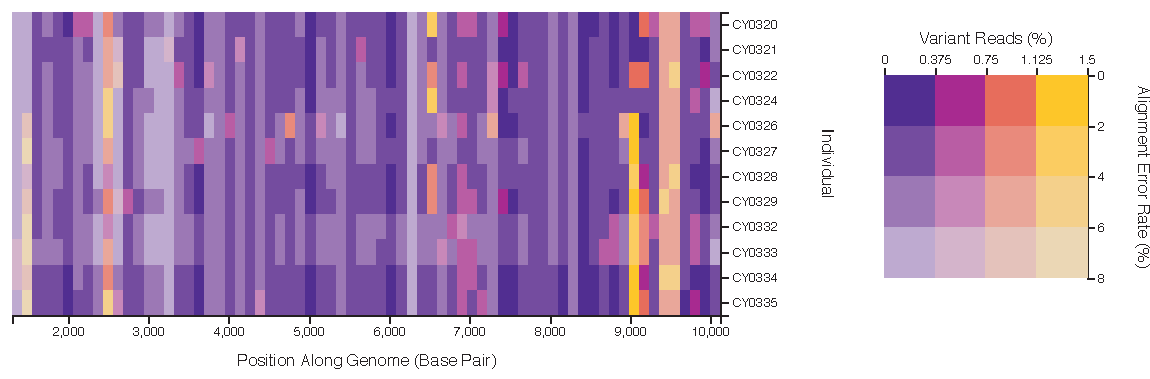
\includegraphics[width=\columnwidth]{viral-2d.pdf}
	\vspace{-15px}
	\caption{Variability for 12 different viral populations of the SIV virus, encoded with a traditional 2D bivariate map. Horizontal position denotes location along the SIV genome. Each row is the viral population of a different infected animal. Error in aligning short reads can lead to poor quality data, and so the amount of these errors is encoded as the uncertainty. }
	\label{fig:viral2d}

	\vspace{10px}

	\centering
	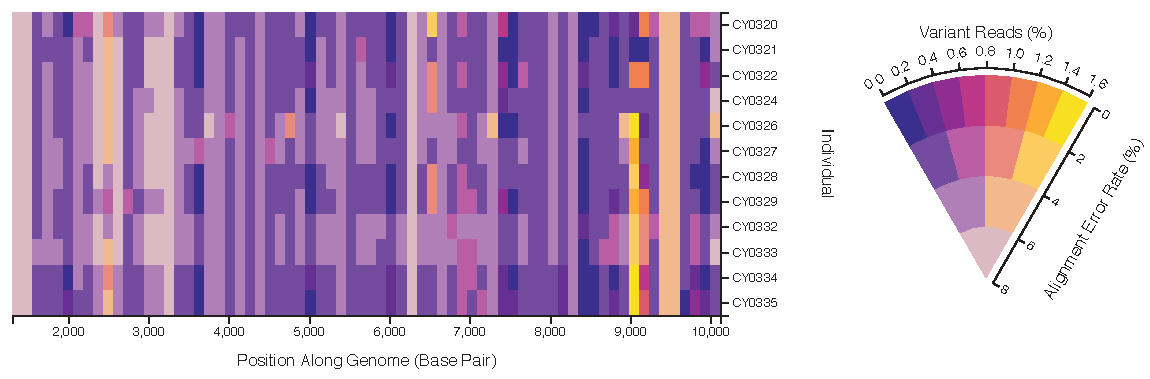
\includegraphics[width=\columnwidth]{viral-vsum.pdf}
	\vspace{-15px}
	\caption{Variability for 25 different viral populations of SIV, encoded with a VSUM. The magnitude of mutation rate, as well as the generally poorer quality of data towards the end of the sequence, is more readily visible than with the traditional bivariate color map. }
	\label{fig:viralVsum}
\end{figure}
}

\newcommand{\responseTimeFig}{
	\begin{figure}[t]
		\centering
		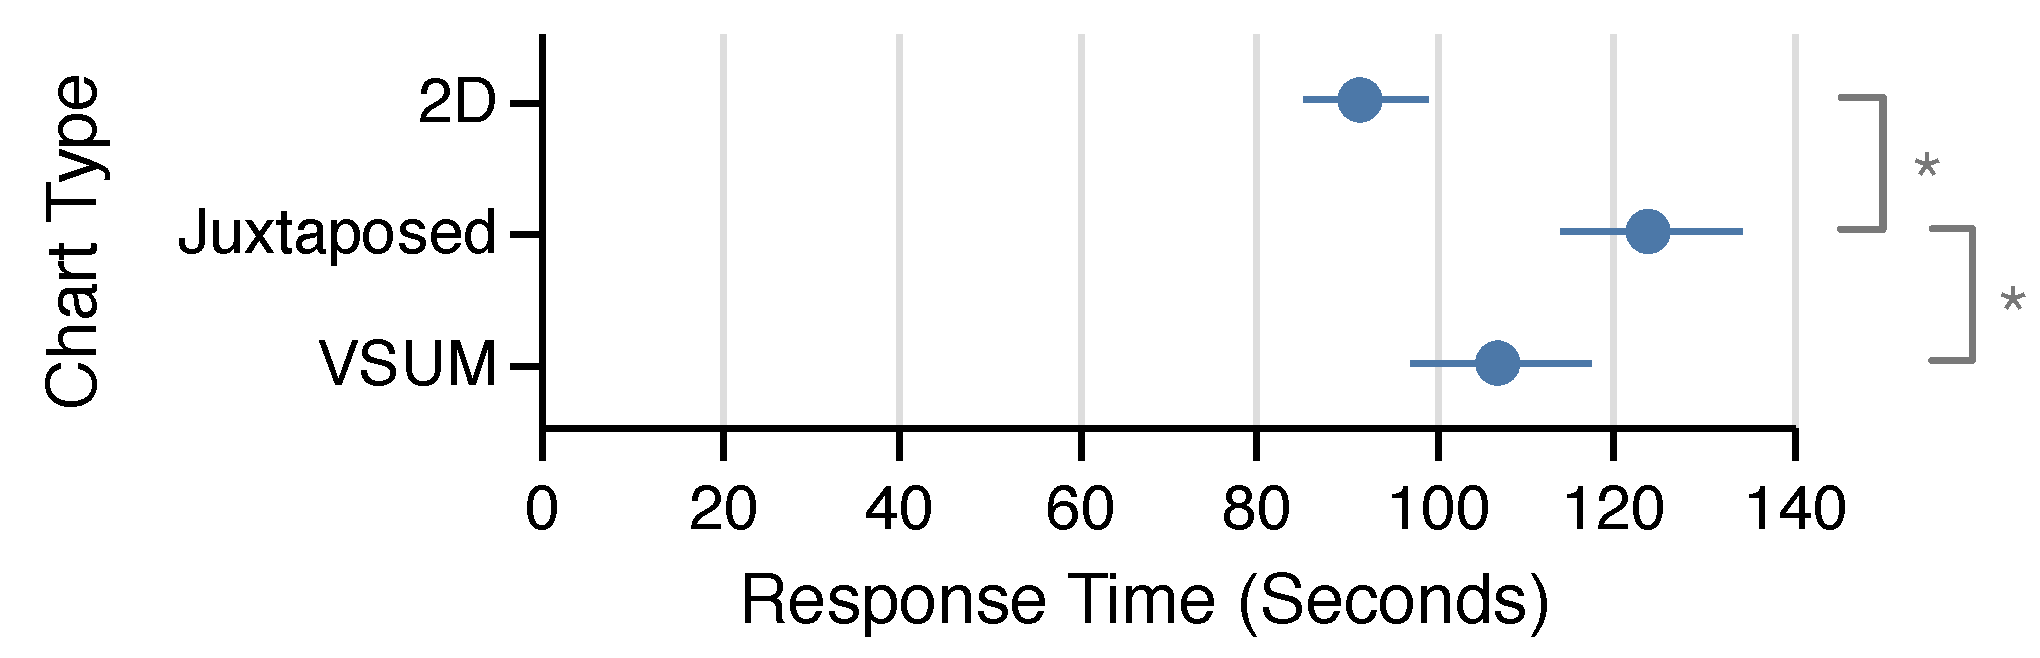
\includegraphics[height=2.4cm]{rt1.pdf}
		\caption{The effect of chart type on response time for the identification task. Juxtaposed maps of value and uncertainty introduce a visual search task, increasing the time to complete even simple tasks involving both value and uncertainty information. The confidence intervals are bootstrapped 95\% CIs of trimmed means.}
		\label{fig:rt1}
	\end{figure}
}

\newcommand{\accuracyFig}{
	\begin{figure}[t]
		\centering
		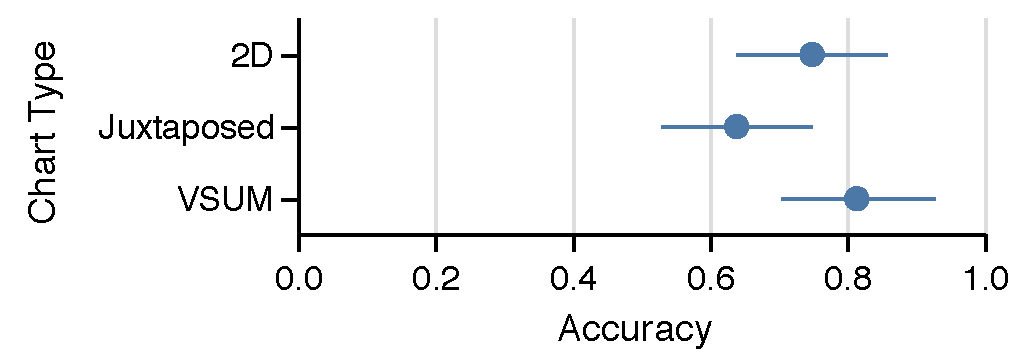
\includegraphics[height=2.4cm]{accuracy1.pdf}
		\caption{The effect of chart type on accuracy for the identification task. VSUMS are similarly accurate for simple search tasks as more traditional bivariate visualizations, despite containing additional colors categories, and having a more complex relationship between uncertainty, value, and color than traditional charts. The confidence intervals are bootstrapped 95\% CIs of trimmed means.}
		\label{fig:accuracy1}
	\end{figure}
}

\newcommand{\uncertaintyFig}{
	\begin{figure}[t]
		\centering
		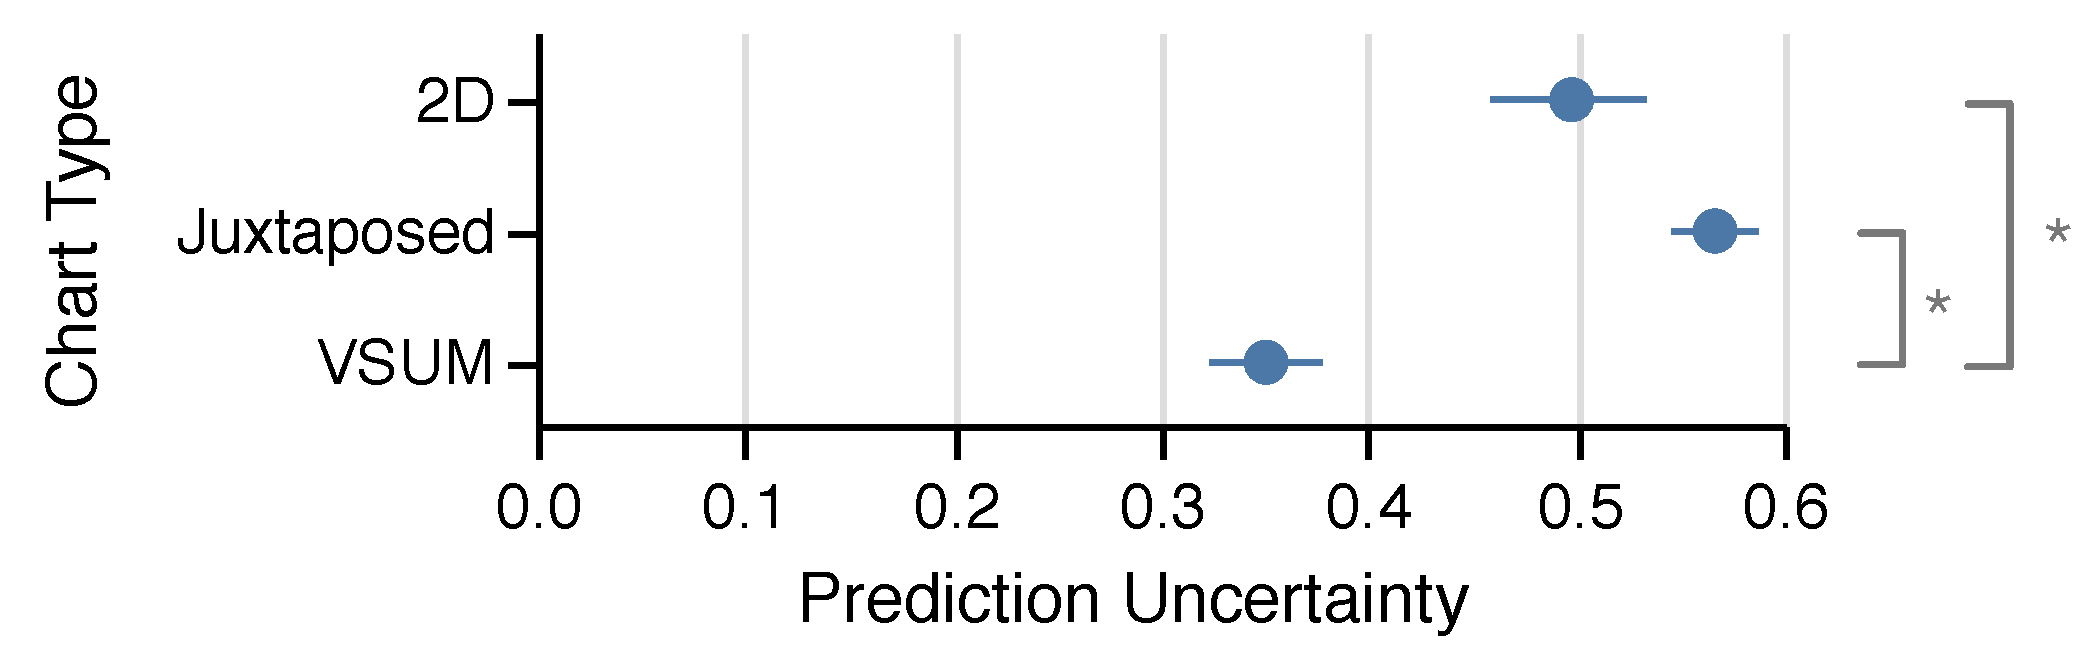
\includegraphics[height=2.4cm]{uncertainty2.pdf}
		\caption{The effect of chart type on the average uncertainty in predictions for the prediction task. By reducing the number of color categories as uncertainty increases, VSUMs encourage more caution in predictions, making people less likely to consider data with strong, but spurious patterns. The confidence intervals are bootstrapped 95\% CIs of trimmed means.}
		\label{fig:uncertainty2}
	\end{figure}
}

\newcommand{\strategyFig}{
	\begin{figure}[t]
		\centering
		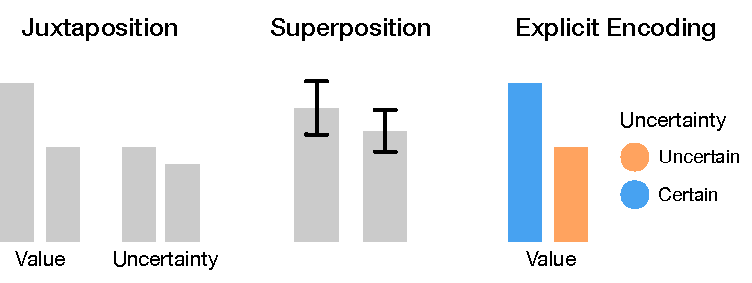
\includegraphics[width=.9\columnwidth]{strategies.pdf}
		\caption{Strategies for encoding uncertainty information along with values. From left to right: encode uncertainty is a separate visualization, overlay uncertainty information, or encode uncertainty with a separate channel.}
		\label{fig:strategies}
	\end{figure}
}

\numberofauthors{3}
\author{%
  \alignauthor{Michael Correll\\
    \affaddr{Tableau Research}\\
    \email{mcorrell@tableau.com}}\\
  \alignauthor{Dominik Moritz\\
    \affaddr{University of Washington}\\
    \email{domoritz@cs.washington.edu}}\\
  \alignauthor{Jeffrey Heer\\
    \affaddr{University of Washington}\\
    \email{jheer@uw.edu}}\\
}

\maketitle

\begin{abstract}
  Understanding uncertainty is critical for many analytical tasks. 
  One common approach is to encode data values and uncertainty values independently, using two visual variables. These resulting bivariate maps can be difficult to interpret, and interference between visual channels can reduce the discriminability of marks.
  To address this issue, we contribute Value-Suppressing Uncertainty Palettes (VSUPs). VSUPs allocate larger ranges of a visual channel to data when uncertainty is low, and smaller ranges when uncertainty is high. This non-uniform budgeting of the visual channels makes more economical use of the limited visual encoding space when uncertainty is low, and encourages more cautious decision-making when uncertainty is high. 
  We demonstrate several examples of VSUPs, and present a crowdsourced evaluation showing that, compared to traditional bivariate maps, VSUPs encourage people to more heavily weight uncertainty information in decision-making tasks.
  
\end{abstract}

\category{H.5.0.}{Information Interfaces and Presentation
  (e.g. HCI)}{General}

\keywords{\plainkeywords}

%

\section{Introduction}
\exampleFig

Uncertainty is an inescapable component of collecting, analyzing, and presenting data. A common goal in the communication of uncertainty is promoting \emph{uncertainty-aware decisions}: the audience should be aware of the risks and rewards of certain decisions, modulate their confidence in their conclusions, and perhaps refrain from making a decision at all if there is too much uncertainty.  A way that designers can contribute to this goal is by ensuring that uncertainty information is \emph{well-integrated} with the rest of the data. That is, it should be difficult to discount or ignore the uncertainty in a dataset.

Simultaneous presentation of uncertainty and value necessitates the construction of a bivariate map\,---\,a relation, in terms of visual variables, between 2-tuples $(\text{value}, \text{uncertainty})$ and mark properties. Due to the interference and interplay between different visual variables, bivariate maps may suffer from limited discriminability.

In this paper, we contribute \textbf{Value-Suppressing Uncertainty Palettes} (VSUPs) for integrating data and uncertainty information in visualizations.
VSUPs intentionally alias together data values with high uncertainty, affording greater discriminability as uncertainty decreases. Traditional bivariate maps might be thought of as a 2D square, with differing outputs for each combination of value and uncertainty. In contrast, VSUPs can be conceptualized as arcs: as uncertainty increases, values are mapped to smaller and smaller sets of outputs, culminating in a singularity where all inputs are mapped to an identical, highly uncertain mark regardless of data value. \figref{fig:example} shows examples of both a traditional bivariate map and a VSUP.

We describe the motivations for VSUPs, provide examples of their utility for decision-making under uncertainty, and assess VSUPs in a crowdsourced experiment. Our results indicate that VSUPs create close integration between uncertainty and data. This integration has a demonstrable effect on decision-making, leading viewers to make more cautious choices that avoid high uncertainty.

\section{Related Work}

% What this section needs to do:
% State of the art in uncertainty vis, with heavy emphasis on MacEachren & co.
% Bivariate maps are hard!
% Binning colormaps is de rigueur
% The variables we'd want to use for uncertainty (like value or alpha or size) mess with color discriminability

Despite the acknowledged importance of uncertainty in understanding data, explicit representations of uncertainty are often missing from visualizations~\cite{boukhelifa2009uncertainty}. This is partially due to the complexity of uncertainty as a concept. In typologies from Thomson \ea~\cite{thomson2005typology} and Buttenfield \& Beard~\cite{buttenfield1994graphical}, the authors note that many, occasionally contradictory, concepts can fall under the category of ``uncertainty,'' including data quality, sampling error, credibility, and provenance.

%There are many methods for visualizing uncertainty. MacEachren \ea~\cite{maceachren1992visualizing} present a theoretical survey of uncertainty visualization. Relevant to our domain of heatmaps and thematic maps \textbf{JH: where did this come from? There is no mention of focusing on this domain in the intro. The whole carto/GIS stuff seems to come out of left field.} is work in GIS and cartography; for a survey of uncertainty visualization techniques in GIS, see Kinkeldey \ea~\cite{kinkeldey2014assess,kinkeldey2017evaluating}. Yet, despite a wide variety of methods, to our knowledge, there are no established standards for visualizing uncertainty in heatmaps.

Reviewing the state of the art in uncertainty visualization in the field, Greithe \ea~\cite{griethe2006visualization} and Brodlie \ea~\cite{brodlie2012review} present lists of potential techniques for conveying uncertainty in concert with data. Some of these options (interaction, animation, and sonification) are not applicable for static charts; even for dynamic charts, many users do not interact with charts in sufficient detail to recover uncertainty information~\cite{nyt2016}. While we acknowledge the potential utility of these techniques in uncertainty visualization (for instance, the animation used to convey sampling error in Hullman \ea's Hypothetical Outcome Plots~\cite{hullman2015hypothetical}), we limit the scope of our discussion to techniques which center on static charts.

\subsection{Visual Variables for Uncertainty}

% 1d uvis: olston2002visualizing, wickham201140, neyman1937outline

One challenge of uncertainty visualization is that the decision to explicitly encode uncertainty increases the dimensionality of the data, and so requires the use of (at least one) additional visual channel~\cite{brodlie2012review}. Uncertainty therefore inherently increases the visual complexity of a visualization. When the data are already complex to convey, and many of the more common or accurate visual variables are in use, allocating an additional dimension is non-trivial. As the number of dimensions increases, finding visual variables that are both perceptually accurate (in either estimation of quantity or discrimination of category) as well as perceptually separable from all the other encoding channels, becomes increasingly difficult. 

A further hurdle is that not all visual variables are well-suited for conveying uncertainty. MacEachren \ea~\cite{maceachren2012visual} evaluate a number of visual variables with respect to their \emph{semiotic fit} for representing uncertainty. They observe that certain visual variables such as blurriness and transparency seem to have a more intuitive connection to uncertainty than other variables such as shape or hue. Unfortunately, Boukhelifa \ea~\cite{boukhelifa2012evaluating} find that many visual variables habitually used for conveying uncertainty, such as blur and value, are also difficult to estimate. This results in a preference/performance gap where designers must choose between encoding uncertainty in a way that is intuitive but error prone, or use higher fidelity channels that may not intuitively convey uncertainty.

\subsection{Bivariate Maps}

While uncertainty can be visualized entirely separately from the rest of the data (for instance, in a juxtaposed chart), this runs the risk that uncertainty information becomes \emph{ignorable}~\cite{moritz2017trust}. It also complicates analysis, as interpreting the value and uncertainty of a given data point requires consulting two separate charts. To integrate uncertainty information into an analysis, we focus on the construction of \emph{bivariate maps}, where value and uncertainty information is displayed simultaneously in a spatially co-located manner.

Bivariate maps can, in principle, be constructed from the combination of any two visual variables (such as shape and color, or size and texture). For example Ware's ``textons''~\cite{ware2009quantitative} overlay glyphs on top of regions to simultaneously encode two quantitative values. However, for spatial visualizations like choropleth maps, heatmaps, and treemaps, visual channels such as position and length are reserved for data variables other than value (such as geographic location or relative size). In these situations, data value is often encoded using color. Bivariate maps in these settings therefore typically rely on a visual channel related to color for encoding a secondary variable, such as opacity~\cite{roth2010value} or pixel noise~\cite{lucchesi2017visualizing}.

Colors in univariate quantitative color maps should be sufficiently far apart as to be perceptually distinguishable~\cite{ware1988color}, and vary in lightness as well as hue to afford an implicit ordering of value~\cite{borland2007rainbow,rogowitz2001blair}. Different choices of color maps can highlight different features of the data, and should be chosen with care~\cite{rogowitz1996not}. These principles extend to bivariate color maps, with the additional consideration that our perception of color channels lacks \emph{orthogonality}. That is, while we can perceive e.g., the height of a bar in a bar chart independently of its width, a particular property of a color (e.g., its redness, saturation, transparency, etc.) affect how its other properties are perceived \cite{garner1970integrality,ware2012information}. Many color channels such as hue and saturation are therefore perceptually \emph{integral}, which complicates their use in bivariate maps.

Another recurring design consideration when constructing color maps is whether to quantize data into a discrete set of colors, or to encode data using a continuous mapping. While continuous color maps afford greater fidelity in presenting values~\cite{muller1979perception}, non-linearity in human color perception introduces errors in extracting numeric values from continuous colors~\cite{borland2007rainbow}. Quantizing a color map is therefore an exercise in balancing \emph{perceptual} error and \emph{quantization} error~\cite{dobson1973choropleth}. Discrete maps offer finer control over this balance, which can result in better performance in tasks involving heatmaps~\cite{padilla2017evaluating}.

In general, the quality of bivariate color maps is a multivariate measure involving consideration of not just the component color channels, but also the interpolation scheme and the color of the surround~\cite{bernard2015survey}. However, even simple bivariate maps can be difficult for a general audience to interpret: due to their additional complexity, Wainer \& Francolini~\cite{wainer1980empirical} reported high levels of error for participants even for ``elementary'' graph reading tasks, and additionally that bivariate legends were more difficult to memorize and internalize than their univariate equivalents. Therefore, bivariate maps in practice are often limited to a small set of output colors~\cite{robertson1986generation,trumbo1981theory} (say, a 4x4 matrix as in \figref{fig:example}).

Given that bivariate maps, for reasons of either practicality or perceptual fidelity, have only a limited budget of outputs, we adapt an insight from Dunn~\cite{dunn1989dynamic} that these limited categories ought to be assigned with regards to their importance to analysis tasks, rather than uniformly. Our Value-Suppressing Uncertainty Palettes apply this insight to data with uncertainty. Frequently, uncertain information ought to be weighted less heavily in a decision-making process, or at least have less prominence in an analysis, than information with high certainty.

Correll \ea~\cite{correll2015layercake,correll2011visualizing} use a precursor of VSUPs in their LayerCake genomics visualization tool, where marks representing genomic data with increasing uncertainty are mapped to a smaller and smaller set of increasingly grey colors, creating the effect of uncertain values retreating into a ``confidence fog'' while highly certain values remain prominent. Other bivariate visualizations implicitly alias together uncertain values through perceptual integrality. For instance, if uncertainty is encoded by transparency, a maximally uncertain glyph may be entirely transparent, and so impossible to distinguish from any other maximally uncertain glyph. Other channels with a semiotic connection to uncertainty, such as saturation, value, blur, or size, have similar deleterious effects on the disambiguation of colors and shapes. In both cases, the property of aliasing is \emph{ad hoc}, and places no guarantees on the discriminability of colors. The binning and degradation approach of VSUPs makes the choice to alias values explicit to both the designer and the viewer, and results in a bivariate mapping with known perceptual properties.

\section{Value-Suppressing Uncertainty Palettes}
Value-Suppressing Uncertainty Palettes (VSUPs) are a technique for creating bivariate maps of data \emph{value} and \emph{uncertainty}. VSUPs make two central assumptions about bivariate maps:

\begin{enumerate}
	\item There is a limited \emph{budget} for perceptual discriminability.
	\item Differences among \emph{certain} data are more germane than differences among \emph{uncertain} data.
\end{enumerate}

In some cases, these assumptions are violated. For instance, an analyst might be interested in ``long tail risks'' or other ``black swan events,'' where the impact of a value, no matter how uncertain, must be considered and planned for~\cite{taleb2011black}. Other analysis tasks (such as filtering out outliers), require increased, rather than decreased, discriminability when uncertainty is high. However, for many information fusion tasks, the assumption is that uncertainty is related to data quality, or the uncertainty of data values~\cite{riveiro2007evaluation}.

If both of these assumptions hold, then it follows that the designer of a bivariate map should allocate more mark types to certain values, and fewer mark types to uncertain values. VSUPs codify this decision by \emph{reducing the number of mark categories for representing value as uncertainty increases.} This means that data encoded using a VSUP will make visible only the largest of differences in uncertain data, but highlight comparatively small differences in value when uncertainty is low. VSUPs therefore act as both a filtering mechanism (in that values with too much uncertainty are mapped to the same glyph), as well as an implicit test of effect size (in that smaller and smaller changes in value are visible as uncertainty decreases). This strategy of dampening low quality or highly uncertain values in maps in order to focus on more informative regions has measurable benefits, including the removal of statistically spurious visual patterns, and the highlighting of regions of interest~\cite{correll2017surprise}.

VSUPs rely on an underlying \textbf{quantization tree} that governs how values are discretized. Values above a certain uncertainty threshold are mapped to a singular ``root'' node. As uncertainty decreases, the tree branches into leaves, which evenly divide the data domain. The data value of a parent is the midpoint of all of its children. These leaves can then branch again, up to a designer-specified stopping point. The layers quantize the uncertainty domain, and sibling nodes quantize the data domain. \figref{fig:example} shows a VSUP with a tree with a branching factor of 2 and 4 layers, resulting in an output range with 15 distinct colors.

Since the visual channel used to encode uncertainty (e.g., saturation, lightness, transparency) often reduces the ability of people to distinguish colors, VSUPs have the added benefit of creating bivariate palettes that are perceptually easier to distinguish, by reducing color resolution in precisely the areas where color disambiguation would be most difficult anyway. For instance, the two closest colors in the VSUP in \figref{fig:example} are 1.4 units farther apart in CIELAB color space than the two closest colors in the traditional bivariate map.

JavaScript code for generating VSUPs for use in D3~\cite{bostock2011d3} charts is available at \url{https://github.com/uwdata/spatial-sampling}.

\subsection{Design Considerations}

There are multiple choices that designers must make before creating a VSUP. Specifically, they must choose which visual channels map to value (1), uncertainty (2), and the structure of the underlying VSUP tree (3).

When selecting a visual channel to represent uncertainty, we recommend channels with both a strong semiotic connection to uncertainty (such as those recommended by MacEachren et al.~\cite{maceachren2012visual}) as well as a relatively large number of perceptually distinguishable levels (such as those evaluated by Boukhelifa et al. \cite{boukhelifa2012evaluating}). Here, we focus on a combination of increasing luminance and decreasing saturation, as in Hengl \& Toomanian~\cite{hengl2006maps}. Correll \& Gleicher~\cite{correll2014error} provide evidence that even audiences without statistical training can successfully interpret uncertainty information encoded in these channels.

When selecting a visual channel to represent value, the designer should consider the perceptual integrality of the value and uncertainty visual channels. For instance, we use the Viridis~\cite{viridis} color map frequently in this paper, as many standard color ramps (such as sequential ColorBrewer~\cite{harrower2003colorbrewer} ramps), following usual best practices, interpolate in both hue and luminance~\cite{ware1988color}. This interpolation in luminance interferes with our uncertainty encoding, introducing ambiguity. Ramps such as Viridis, which avoid very light and very dark colors, reduce this ambiguity.

When determining the quantization tree, the design should be careful to avoid having too many output colors. For reasons of memorability and complexity, Wainer \& Francolini~\cite{wainer1980empirical} suggest no more than 16 distinct outputs in bivariate maps. For a binary quantization tree, this results in a maximum tree depth of 4, as seen in \figref{fig:example}. In general, for tasks that require finer-grade distinctions between uncertainty, the depth of the tree could be increased. For tasks involving finer-grade distinctions between value, the branching factor of the tree could be increased. However, these factors increase the number of colors, and so designers should moderate between legend complexity and data fidelity. Beyond these two parameters, non-uniform binning would allow the designer to target particular distributions or important subregions of the data that would otherwise be difficult to visualize in a limited palette, as in Dunn's~\cite{dunn1989dynamic} dynamic bivariate maps. As an additional form of control, prior tools using VSUP-like techniques, such as LayerCake~\cite{correll2015layercake}, allow the analyst to control the bins in the tree through interaction with the color legend.

\section{Examples}

We present a set of examples showing how VSUPs can be applied to real-world datasets. VSUPs allocate color bins asymmetrically amongst value and uncertainty regions, affording greater discriminability in regions of the chart that warrant closer scrutiny, while discouraging exploration of regions with noisy or unreliable signals.


\subsection{Air Travel Delay}

\airlineFig

Using a public data set from the U.S. Bureau of Transportation Statistics~\cite{bts}, we created a heatmap showing average flight delay for different times of the day and days of the week for U.S. carriers in January 2017. We use standard error $\left(\sigma / \sqrt{n}\right)$ as our measure of uncertainty. We created two alternate heatmaps of this delay information. \figref{fig:airline2d} shows a traditional bivariate map, whereas \figref{fig:airlineVsup} shows a VSUP generated under the same constraints.

Both maps illustrate a similar trend: flight delays are shorter towards the beginning of the day, increasing on average over time. The traditional bivariate map affords only a coarse examination of this trend: two visible ``blocks'' of color, early in the day, and later in the afternoon. The VSUP, in contrast, has sufficient color resolution to show a quasi-linear trend. Uncertainty is high only for a few bins for which there are small number of flights, either on the weekends or late at night. The VSUP does not obscure any significant trends in the high uncertainty data, despite having fewer color categories overall.

%\subsection{Viral Mutation}
%\viralFig

%Next generation sequencing allows biologists to collect and analyze large amounts of genomics data. However, these techniques often create data quality issues, as they must align large numbers of potentially ambiguous ``reads'' of relatively small numbers of base pairs. Using a dataset from a group of virologists interested in the population dynamics of viral mutation~\cite{o2012conditional}, we visualized the variability in viral genomes across 12 populations of the simian immunodeficiency virus (SIV). In the dataset here, it is important not only to identify hotspots in the viral genome (locations with high rates of mutation or variability), but also to not be distracted by false positives. The traditional bivariate map (\figref{fig:viral2d}) has many locations with apparent inter-population variance.

%VSUPs (\figref{fig:viralVsup}) enable biologists to explore interesting patterns while deemphasizing noise. Orange hot spots towards the beginning (the second column) and end of the genome (around reference nucleotide $9,500$) could be considered potential regions of interest in the 2D map; in the VSUP these are encoded as highly uncertain and of ambiguous value. In fact, these regions have systematically low coverage; the lack of reliable data for these regions should discourage analysts from giving their apparent pattern equal consideration from the stronger signals elsewhere in the genome.

\subsection{2016 Pre-Election Polling}

\pollFig

Using a public data set from Wikipedia~\cite{wiki}, we collected the statewide polls that were conducted closest to the 2016 U.S. presidential election, we created a choropleth map showing which candidate was leading in the polls. We calculated uncertainty as the size of the lead in terms of margin of error (lead/margin). The AP style guide for reporters suggests that a candidate leading by more than two margins of error is said to be ``significantly ahead'' in the polls~\cite{french1988associated}. As the lead becomes closer to the margin of error, there is more doubt about the electoral outcome.

By providing more color categories when the margin of error was relatively small, the VSUP map shows that, in many of the states leaning towards Hillary Clinton, her lead was quite small. The VSUP map, by limiting inferences about which candidate was leading when the uncertainty is high, also prevents the viewer from making strong claims about the outcome of the election in highly volatile states, even if a state is leaning one way or the other. Given the relative volatility in polling data, this caution is warranted. An additional benefit to the VSUP map is that, as the diverging blue-red color map passes through a central whitepoint, it can be difficult to distinguish between uncertainty levels (which also interpolates to white) in the 2D map. The VSUP's tree-like structure separates these problematic colors: the closest colors in the 2D scale are 2.9 units apart in CIELab space, but the closest colors are 6.2 units apart in the VSUP scale.

\section{Evaluation}
\conditionFig

We performed two crowdsourced experiments on Amazon's Mechanical Turk to evaluate the effectiveness of VSUPs for integrating uncertainty and value information in visualizations. This focus on integration meant that we limited our experimental tasks to scenarios where the participants needed to consider both value and uncertainty before making a decision. Each experiment focused on one of two separate tasks:

\begin{enumerate}
	\item An \textbf{identification} task, where we gave participants charts with value and uncertainty information, and asked them to locate specific regions. E.g., ``click on the region of the chart with a value of $0.1$ and an uncertainty of $0.2$.''
	\item A \textbf{prediction} task, inspired by the game Battleship, where we gave participants charts with both \emph{forecast} and \emph{forecast uncertainty} information, and asked the participants to place tokens on the board in order to minimize danger. E.g., ``place your $5$ ships on the safest locations on the board.''
\end{enumerate}

We limited our population to Turkers from the United States, with a prior task approval rate of at least 90\%. As the experimental tasks required multi-hue color perception, we presented participants with a set of Ishihara plates~\cite{hardy1945tests} as a pre-test, and excluded participants who either misidentified the values in the plates, or who self-reported as having a color vision deficiency (CVD) in the post-test. Based on piloting, we paid participants \$2 for participation, for a target rate of \$8/hour. After completion of the main tasks, we solicited demographic information, including a risk aversion assay from Mandrik \& Bao~\cite{mandrik2005exploring}. Participants from the first experiment were excluded from participating in the second.

Experimental materials, including data tables and stimuli generation code, are available at \url{https://github.com/uwdata/spatial-sampling}.

\subsection{Identification Experiment}

We wished to determine what effects, if any, our various design considerations had on performance at a basic analysis task: using a bivariate legend to interpret a heatmap. There are a number of design decisions to be made even after one has determined which two visual channels will be used to encode value and uncertainty.
In particular:
\begin{enumerate}
	\item Whether or not to \emph{juxtapose} or \emph{superimpose} the data and uncertainty maps.
	\item Whether or not to \emph{discretize} each visual channel, or encode values \emph{continuously}.
	\item Whether or not to use a \emph{square} legend, which gives equal area to each bin, or a \emph{wedge} legend, which reduces in size as uncertainty increases.
	\item If discretizing, whether to employ a \emph{VSUP} or a \emph{standard} quantization scheme.
\end{enumerate}

For the identification task, we gave participants a $5$x$5$ heatmap, and asked them to click on a region of the heatmap that encodes a particular (value, uncertainty) pair. To support comparability across conditions, we chose a set of target pairs such that each target mapped to a unique color across all encoding types. This resulted in (4+4+2+1)=11 valid targets. For each trial, we placed one example of each of these 11 targets randomly in a heatmap; the remaining 13 cells of the heatmap were randomly sampled from this target list. Thus there could be multiple correct locations in each trial, deterring a strategy of looking for ``oddball'' colors. 

We selected this task both as a way of assessing the ability of people to successfully encode and decode values using a bivariate map, and to provide training for the prediction task (since we reused the bivariate maps in that task). We measured performance both in terms of accuracy (did the participant select the correct point) as well as response time.

We recruited 24 participants for this task: $12$ female, $12$ male, ($M_{\text{age}}$= $31$, $SD_{\text{age}}$ = $7.8$). Each of the participants saw the data encoded as each of 8 types of bivariate encoding and legend, with 8 replications, for a total of 64 stimuli. \figref{fig:conditions} shows these factor levels.

\subsubsection{Hypotheses}

We had two initial hypotheses, informed by prior work:

\begin{enumerate}
	\item Juxtaposed maps, by introducing a second search task to the identification task (searching for the proper values in two, rather than one map), would have poorer performance than other conditions.
	\item Continuous maps require more specific and accurate color matching between value and color, and so would have poorer performance than discrete conditions.
\end{enumerate}

We had no strong hypotheses about the shape of the legend (square vs. wedge), but, as the wedge shape makes more uncertain bins in the legend smaller (and thus potentially harder to disambiguate), we included it as a check against VSUPs which explicitly alias uncertain values. For this identification task, which did not involve reasoning with uncertainty, but simply matching colors to a color legend, we also did not have strong hypotheses about performance differences between VSUPs and traditional discrete bivariate maps.

\subsubsection{Results}
\taskOneFig

We performed a repeated measures ANOVA on our results to measure the effect of juxtaposed versus superimposed maps, and continuous versus discrete legends, on accuracy. Participant ID was included as a random effect. \figref{fig:taskOne} shows the performance of each of our 8 conditions.

The results support our first hypothesis. Juxtaposition was a significant effect ($F(1,166)=5.5$,$p=0.02$). A post-hoc t-test confirmed ($t=2.5$, $p=0.01$) that superimposed charts ($M=0.58$, $SD=0.50$) performed significantly better than juxtaposed ($M=0.51$, $SD=0.49$) ones. For our identification task, juxtaposition requires at least two search tasks (one to locate squares with the correct data value, another to locate ones with the correct uncertainty value), which introduces additional error compared to conditions where value and uncertainty are displayed simultaneously. 
%This is reflected also in response times, which, although highly variable, were higher in juxtaposed conditions ($M=19$s, $SD=65$), than the other conditions ($M=13$s, $SD=38$), although this difference was not significant ($t=1.64$, $p=0.1$).

The results also support our second hypothesis. Discretization was a significant effect ($F(1,166)=30$,$p<0.01$). A post-hoc t-test confirmed ($t=6.1$, $p<0.01$) that charts with discrete bins ($M=0.63$, $SD=0.48$) performed significantly better than charts with continuous color maps ($M=0.47$, $SD=0.5$). The lack of quantization bias in continuous maps is countered by the perceptual error in precisely estimating value from color. Relying on a discrete set of output colors simplifies this task.

We performed a second ANOVA among the superimposed discrete charts to determine the effect of legend shape (wedge or square) and quantization scheme (VSUP or standard) on performance, with participant ID as a random factor. We did not find a significant effect for either the legend shape ($F(1,70)=0.04$, $p=0.84$) or the quantization scheme ($F(1,70)=1.4$, $p=0.24$).

\subsection{Prediction Experiment}

\taskTwoFig

For the prediction task, we gave participants the rules of a game similar to Battleship. Greis \ea~\cite{greis2016decision} employ these game-like experimental tasks to assess how different visual designs communicate uncertainty information, which can be abstract or complex, to the general audience. In our task, the participant and a (fictional) adversary have to place tokens representing ships on a $5$x$5$ spatial grid, with the expectation that certain squares will be hit by missiles. Players have to place all their tokens before continuing. The objective is to minimize the number of your own ships that are hit. In our task, participants were given a map representing the predictions of missile strikes in each location on the grid. The \emph{value} component was the ship's \emph{danger} if placed on the square. The \emph{uncertainty} component was the confidence in this prediction. Other studies of uncertainty representation, such as in Cox et al.~\cite{cox2013visualizing}, have used "prediction + prediction uncertainty" stimuli to elicit differences in decision-making between visualizations of uncertainty.

Our stimuli were created by randomly sampling from values that fell within each of the $16$ bins of the $4$x$4$ 2D bivariate color map. This resulted in 16 samples. The remaining 9 samples were ``bad'' values, with low safety and high certainty. This created 4 quartile categories of uncertainty, with a skew towards the highest quartile. This stimuli design meant that, while participants had at least one ``safe'' square (low danger with high certainty), they were forced to make at least some guesses in other quartiles.

We selected this task in order to promote risk-averse behavior. Tversky \& Kahneman~\cite{tversky1985framing} illustrate that framings in terms of gains or losses produce reliably different outcomes. In particular, there is greater perceived value in avoiding large losses as opposed to striving for a large gain~\cite{kahneman1979prospect}. Our results from the prior study indicate that discrete, non-juxtaposed maps outperformed the other bivariate maps we selected, so we limited our study to only 4 types: square and wedge bivariate maps. While other map types might produce different patterns of decision-making (for instance, the juxtaposed map might encourage participants to ignore uncertainty information altogether), their low accuracy for our previous information fusion tasks led us to discard them, as it would be difficult to distinguish between different patterns of predictions caused by the design, and different patterns caused by simply misreading the heatmap. Having fewer conditions also afforded a within-subjects design that controlled for the variation in interpersonal differences in strategies and risk-aversion, while limiting the potential effects of learning and fatigue on predictions from large numbers of stimuli.

The ideal strategy from a value-maximizing standpoint would be to place tokens on areas with the lowest predicted danger (highest expected value), ignoring the uncertainty information. However, as with roulette and other similar games of chance, the \emph{variability} in expected value is relevant when considering where to place bets~\cite{mlodinow2009drunkard}. A risky player would choose guesses with high expected value, regardless of the uncertainty of those points. A more conservative guesser might eschew high-risk, high-reward locations, resulting in a lower average value of guesses, but also lower uncertainty. We therefore measured the distribution of both \emph{value} and \emph{uncertainty} of the tokens placed by the participants.

 We recruited 24 participants for this task: $12$ female, $12$ male, ($M_{\text{age}}$= $37$, $SD_{\text{age}}$ = $9.8$). Our selected square and wedge maps were either VSUPs or traditional bivariate maps, for a 2 (square or wedge legend) x 2 (VSUP or standard) factorial design, with 6 replications, for a total of 24 stimuli. Prior to the main task, we included a short replication of the identification task from the prior experiment (with 12 stimuli) for training and exclusion purposes. 3 people with unacceptably low accuracy on the training task ($6\%$, $6\%$, and $25\%$ accuracy compared to a mean of $70\%$) were excluded from analysis. 

\subsubsection{Hypotheses}

We had two hypotheses, stemming from our belief that VSUPs promote better \emph{integration} between uncertainty and value information, and encourage \emph{caution} by highlighting the ambiguity introduced by uncertain data. In particular:
\begin{enumerate}
	\item Participants would avoid targets with \textbf{high uncertainty} when using a VSUP.
	\item This would result in a tradeoff where they would also choose targets with lower expected value \textbf{higher danger} when using a VSUP.
\end{enumerate}

As with the prior experiment, we had no strong hypotheses for square vs. wedge-shaped legends, but included both as a check against the potential implicit VSUP-like properties of wedge-shaped legends.

\subsubsection{Results} 
\taskTwoHeatmap

Consistent with our first experiment, we found no significant effect of legend shape on either uncertainty ($F(1,61) = 0.01$, $p=0.92$) or value ($F(1,61)=3.1$, $p=0.08$) of guesses. This result suggests that wedge- and square-shaped legends promote similar patterns of decision-making. Overall, we prefer to employ the wedge-shaped legend for VSUPs, and the square-shaped legend for traditional maps, as it makes the conceptual differences between the two more apparent.

The results partially support our first hypothesis. We performed a repeated measures ANOVA on our results to measure the effect of VSUP versus standard quantizations, and square- versus wedge-shaped legends, on average uncertainty in bets. We found no significant effect of quantization scheme on average guess uncertainty ($F(1,61)=0.05$, $p=0.83$). This result indicates that there does not appear to be a uniform pattern of risk aversion between the two scale types. However, given our quartile-based stimuli design, the central tendency of uncertainty would not necessarily capture caution in guesses. To capture differences in this non-normal distribution, and to test our belief that VSUP users would avoid highly uncertain regions, we performed a one-sided two-sample, Kolmogorov-Smirnov test on the distributions of uncertainty in guesses in the VSUP and traditional bivariate conditions. We found a significant difference ($D = 0.5$, $p=0.03$), and an inspection of the distribution shows that participants using VSUPs were less likely to make guesses with very high uncertainty. \figref{fig:taskTwoHeatmap} shows this result.

The results support our second hypothesis. A similar ANOVA for average danger value of guesses found a significant effect of quantization scheme ($F(1,59)=17$, $p<0.01$). A post-hoc t-test confirmed ($t=2.3$, $p=0.02$) that guesses made with VSUPs had significantly higher average danger ($M=0.32$, $SD=0.17$) (and so lower expected value) than traditional maps ($M=0.29$, $SD=0.18$).

These two results, taken together, suggest that VSUPs led participants to moderate their guesses: avoiding highly uncertain regions, but willing to ``gamble'' more on regions of middling certainty. In our design, where these gambles were usually poor (due to the predominance of ``bad'' cells), this moderation resulted in guesses with higher average danger. However, when expected value and uncertainty are orthogonal, this moderation can be beneficial, or at least not harmful. Indeed, for guesses with middling and low uncertainty (quartiles 1-3), where this orthogonality was present, there was no significant difference ($t=1.56$, $p=0.11$) in average danger between VSUP ($M=0.30$, $SD=0.24$) and traditional ($M=0.29$, $SD=0.24$) conditions. 

\section{Discussion}

Our experimental results have a number of implications for designers wishing to employ bivariate maps for encoding uncertainty. Both of our experiments show that the way that uncertainty information is presented can have a measurable impact on decision-making. VSUPs make a number of design choices in presenting uncertainty. Firstly, they present uncertainty information simultaneously (superimposed) with value, rather than in juxtaposed charts. Secondly, they encode value and uncertainty via discrete, quantized bins, rather than continuously. Lastly, they are designed to alias and suppress uncertain values, rather than certain values. Our experiments provide evidence about the potential impact of each of these choices on performance for information fusion tasks. We will discuss the impact of our experimental findings on the consideration of each of these design decisions in turn.

\subsection{Juxtaposition vs. Superposition}

Gleicher et al.~\cite{gleicher2011visual} propose three major categories for visualizations that support comparison: juxtaposition (where two variables are visualized in adjacent charts), superposition (where the two variables are encoded simultaneously in a single chart) and explicit encoding (where the two variables are reduced to a single calculated variable, which is directly visualized). Juxtaposition has a number of advantages for bivariate data of this sort: firstly, there are no issues of the integrality of different components of color perception, as there are separate maps for both uncertainty and value. Secondly, juxtaposed displays allow viewers to separately consider patterns in value and uncertainty. The literature also suggests that superposition, which requires a bivariate scale, results in poor accuracy even for basic identification tasks~\cite{wainer1980empirical}.

However, our results indicate that juxtaposed visualizations have a substantial drawback for information fusion tasks. 


\subsection{Discrete vs. Continuous Encodings}

When using color to encode data, designers must make the decision whether or not to separate the data into discrete classes of color outputs, or to employ a continuous and class-less scale. This, in turn, introduces a trade-off between \emph{quantization error} (the sampling error introduced by binning the data) and \emph{perceptual error} (the error introduced by the viewer as they decode the color). There is also a cost in terms of expressivity and consistency: a designer might wish for quantitative, continuous information to be represented continuously~\cite{mackinlay1986automating}.

However, for bivariate color maps, where often the color properties used to encode value and uncertainty are not perceptually separable, error in decoding values can be quite high.  In our identification experiment, this perceptual error was high. Continuous maps performed the worst of all of our other bivariate map types (47\% vs. 63\% accuracy for discrete maps). This is likely due to the non-linearity of 

\subsection{Risk Aversion vs. Risk Seeking}

It is often difficult for the general audience to successfully make use of uncertainty information.  In order to minimize the complexity of uncertainty, uncertainty information is often visualized in a binary way, where values either meet some explicit uncertainty standard, or do not. These binary encodings for uncertain information, such as error bars for estimates, or ``cones of uncertainty'' for hurricane paths, result in binary patterns of decision-making that do not accurately reflect the underlying uncertainty in the data~\cite{cox2013visualizing,correll2014error}.

We designed VSUPs to promote risk-averse decision-making. In the limit of uncertainty VSUPs have only one output color, and so explicitly prevent any decoding of value. This narrowing of options is reflected not only in the quantization scheme, but also in the shape of the legend, narrowing as the uncertainty increases. This is despite the fact that the continuous maps were constructed via interpolations in CIELAB colorspace, which was designed for perceptual uniformity~\cite{mahy1994evaluation}. 
%\sizeFig


%exp1
%continuous bad
%juxtaposed bad

%exp2
%vsup: more cautious

%The results from our initial evaluation of VSUPs are promising, showing that a general audience can make use of uncertainty information in a reasonable way. The way that uncertainty information is presented can have a measurable impact on decision-making. The VSUP strategy of only emphasizing differences when uncertainty is sufficiently low is somewhat analogous to the inferential statistics such as effects tests. VSUPs might therefore be used to promote more caution in judgments, and lead analysts away from spurious signals in data.

% results to discuss:
% bivariate maps: performance can be bad! esp. compared to univariate maps
% juxtaposition bad
% encourages caution
% different patterns of risk, same people


%Bivariate maps have an inherent limitation in that visual channels are often difficult to attend to separately or orthogonally. Bivariate maps are also complex to interpret. Systems which simultaneously display large amounts of value and uncertainty data to general audiences (such as Pangloss~\cite{moritz2017trust}) avoid them for precisely these reasons, relying instead on juxtaposed maps. Our results indicate that juxtaposition produces additional problems, forcing users that wish to integrate uncertainty and data to locate an item of interest, and then re-locate that same item in a visually distant map, which may have few visual landmarks in common. This additional step before information fusion is reflected in longer response times, and patterns of decision-making that are less mindful of risk.

\subsection{Limitations and Future Work}

VSUPs assume that uncertain values ought to have less visual impact that highly certain values. VSUPs therefore act both as a kind of filtering device as well as a bivariate representation. This assumption holds in scenarios like the polling dataset (\figref{fig:pollingVsup}), where the expectation is that highly uncertain data is unreliable or should otherwise be downweighted in analysis. If the analyst has a different interpretation of uncertainty, or wishes to quickly and orthogonally analyze the distributions of uncertainty and value, other strategies, such as juxtaposed maps, may be more appropriate. VSUPs are designed for the \emph{integration} of value and uncertainty. Designers should take care in considering when and how this integration is desirable.

Our experiments dealt with cases where both uncertainty and value were represented by color. The perceptual non-separability of color channels is well-known~\cite{garner1970integrality, ware2012information}, and so the concept of a limited ``budget'' of distinguishable marks easier to quantify and illustrate. In principle, a VSUP can be created for any combination of visual variables. All that is required is a perceptual model of the interaction between these two variables. Where these models exist, as with the interaction between size and color~\cite{stone2014engineering}, the creation of VSUPs is straightforward. Where these models do not exist, or where the perceptual interaction is too complex to efficiently model, experimental work remains to be done before VSUPs can be considered a feasible design strategy. We are currently experimenting with the creation of VSUPs using these other channels, such as color and size.

VSUPs, like other mappings involving quantization, are also highly sensitive to the binning scheme used. Uncertain data with values that fall very close to bin boundaries may end up having large color differences, even though they may be close in value. The comparison to effects tests is therefore imperfect, and a particular item's encoding in a VSUP cannot be used as a proxy for a test of statistical significance. As with other quantized forms of data analysis, including histograms and geospatial binning, analysts and designers should consider the distribution of values before quantizing.

\subsection{Conclusion}

Uncertainty, data quality, or confidence values are often considered separately from the data itself, relegated to tooltips or visually distant supplemental charts. We contend, in contrast, that uncertainty information ought to be directly integrated within a shared chart. This integration introduces additional complexity in the design and presentation of data. Value-Suppressing Uncertainty Palettes represent one strategy for dealing with this complexity, by assigning mark properties in a way that supports the disambiguation of values in data where uncertainty is low, but suppresses these judgments when uncertainty is high. This decision of how to allocate visual variables promotes patterns of decision-making that make responsible use of uncertainty information, discouraging comparison of values in unreliable regions of the data, and promoting comparison in regions of high certainty.

\section{Acknowledgments}

This work was supported by a Moore Foundation Data-Driven Discovery Investigator Award.


% BALANCE COLUMNS
\balance{}

% REFERENCES FORMAT
% References must be the same font size as other body text.
\bibliographystyle{SIGCHI-Reference-Format}
\bibliography{uncertainty}

\end{document}

%%% Local Variables:
%%% mode: latex
%%% TeX-master: t
%%% End:
